
\chapter{Black hole-galaxy co-evolution in the context of quenching}\label{chap:agn}

The following chapter is split into two parts; in Section \ref{agnfeedback} I investigate the connection between quenching parameters and the presence of an AGN and in Section \ref{intbulgeless} investigate how black holes grow in disc galaxies with merger free evolutionary histories. 

\section{Rapid, recent quenching within a population of Type 2 AGN host galaxies}\label{sec:agnfeedback}

\emph{The work in the following chapter has been published in \citet{smethurst16}.}

In Chapter \ref{morph}, rapid quenching rates were dominant across the smooth weighted population densities in Figures~\ref{green_v} \& \ref{red_s}. In Section~\ref{rapid} I discussed how simulations suggest that such rapid quenching rates can only be achieved if AGN feedback is present in a major merger scenario. I therefore decided to investigate this possible connection between AGN feedback and rapid quenching rates further. I shall do so by analysing the SFHs of a population of AGN host galaxies with \textsc{popstarpy} in comparison to an inactive galaxy control sample. I  aim to determine the following: (i) Are galaxies currently hosting an AGN undergoing quenching? (ii) If so, when and at what rate does this quenching occur? (iii) Is this quenching occurring at different times and rates compared to a control sample of inactive galaxies? This builds on the work of \citet{Martin07} but improves significantly on previous techniques.

\subsection{AGN Sample}\label{agnsample}

\begin{figure*}
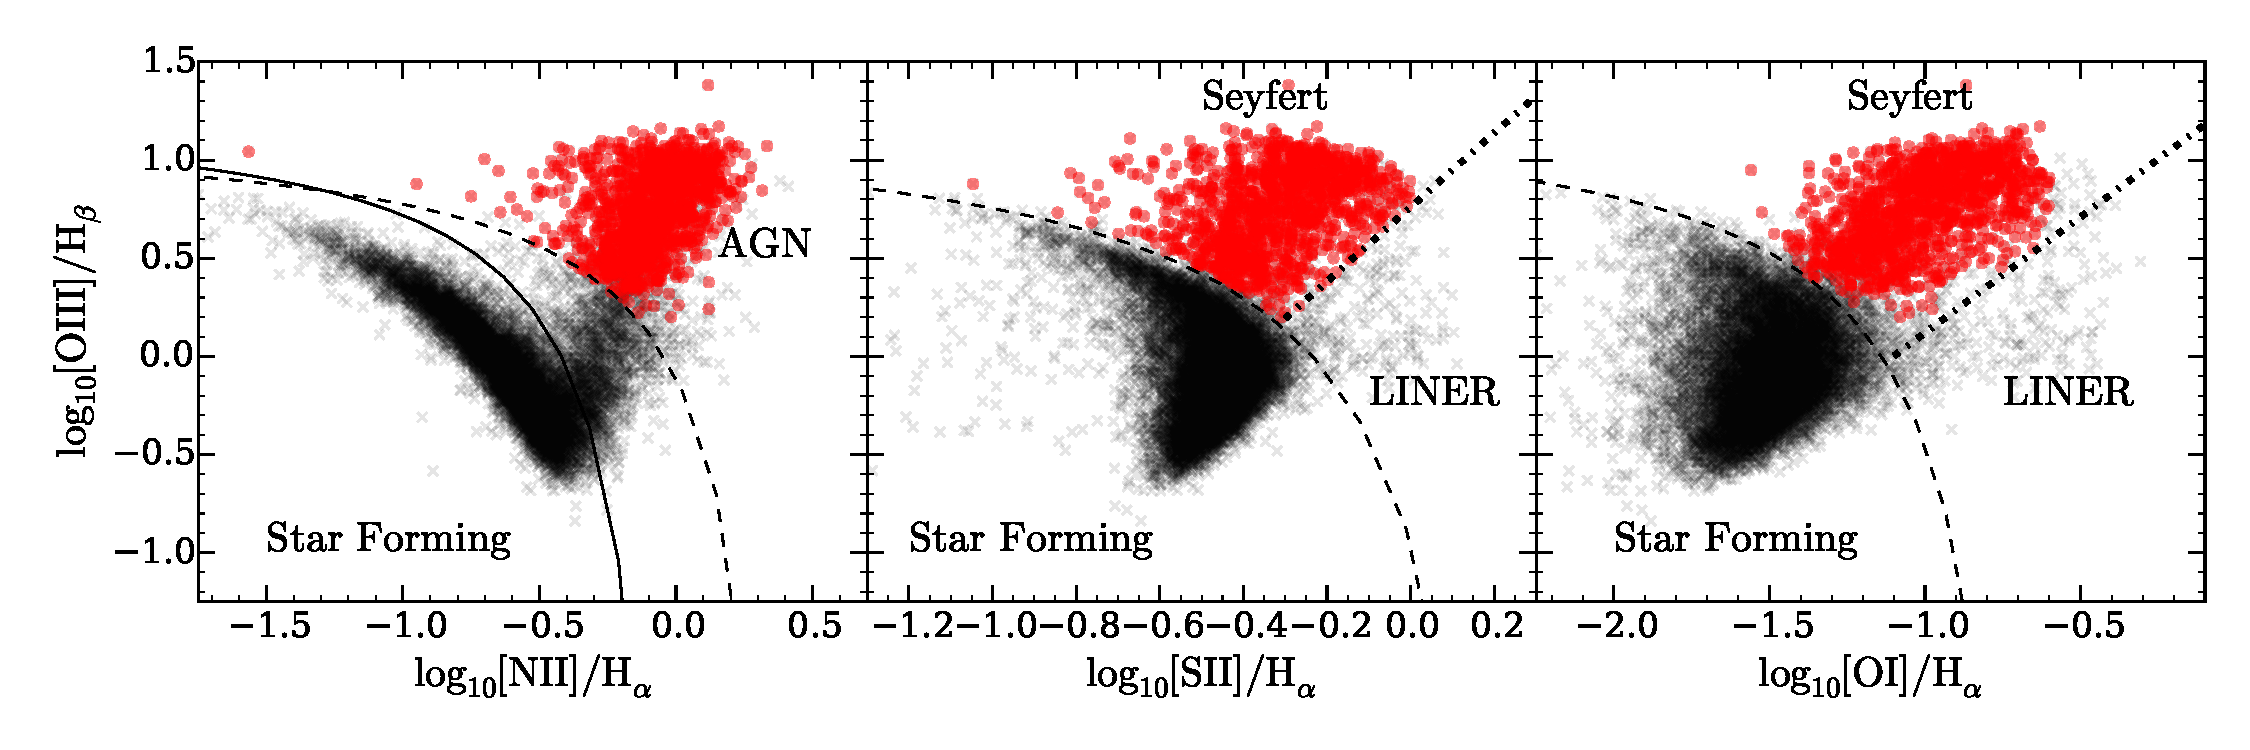
\includegraphics[width=\textwidth]{agn/fig2.pdf}
\caption[BPT diagram used to select AGN host galaxies]{BPT diagrams for galaxies in the \textsc{gz2-galex} sample (black crosses) with S/N $> 3$ for each emission line. Inequalities defined in: \protect\cite{kewley01} to separate SF galaxies from AGN (dashed lines), \protect\cite{kauffmann03b} to separate SF from composite SF-AGN galaxies (solid line) and \protect\cite{kewley06} to separate LINERS and Seyferts (dotted lines). Galaxies are included in the \textsc{agn-host} sample (red circles) if they satisfy all the inequalities to be classified as Seyferts. LINERs are excluded for purity.}
\label{bpt}
\end{figure*}

\begin{figure*}
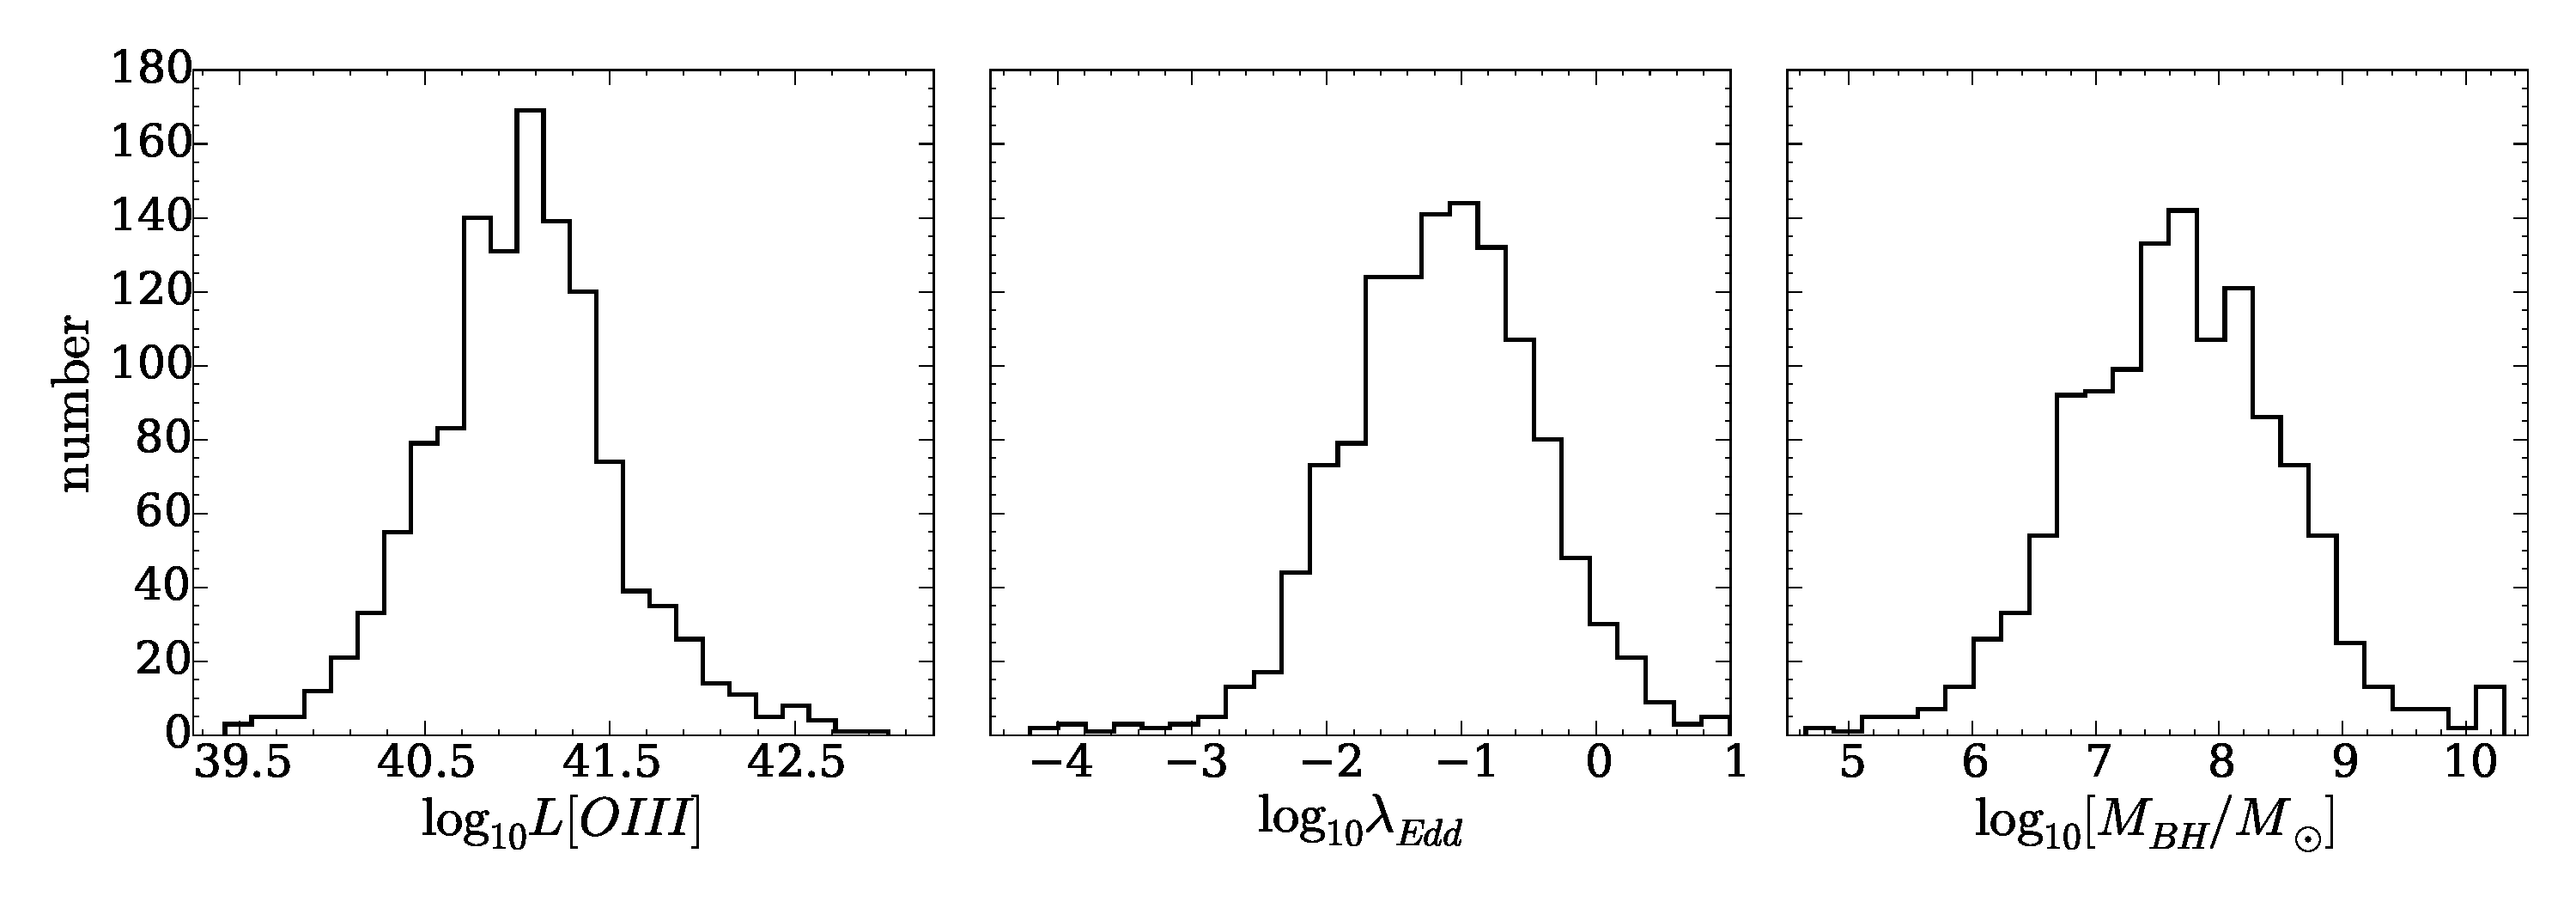
\includegraphics[width=\textwidth]{agn/agn-host_distributions_loiii_edd_ratio_mbh.pdf}
\caption[Distribution of measured galaxy parameters in the \textsc{agn-host} sample]{Distribution of the [OIII] luminosity (left), Eddington ratio (middle) and black hole masses (right) in the \textsc{agn-host} sample.}
\label{fig:agndistributions}
\end{figure*}


Type 2 AGN were selected from the \textsc{gz2-galex} sample using a BPT diagram \citep{bpt} using line and continuum strengths for [OIII], [NII], [SII] and [OII] obtained from the MPA-JHU catalogue \citep{kauffmann03, brinchmann04}. A BPT diagram uses emission line ratio diagnostics to determine whether a galaxy is a star forming galaxy, a Seyfert (i.e. hosting an AGN) or a LINER. The signal-to-noise ratio was required to be S/N $> 3$ for each emission line as in \cite{schawinski10a}. Those galaxies which satisfied all of the inequalities defined in \citet[][to separate SF galaxies from AGN]{kewley01} and \citet[][to separate SF galaxies from composite SF-AGN galaxies]{kauffmann03b} were selected as Type 2 AGN, giving $1,299$ host galaxies ($\sim10\%$ of the \textsc{gz2-galex} sample; in agreement with estimates of the local AGN fraction of \citealt{kauffmann04, pimbblet13}).

\cite{Sarzi10, yan12} and \cite{Singh13} have all demonstrated that LINERs are not primarily powered by AGN, therefore for purity, these galaxies were excluded from the sample using the definition from \cite[][$55$ galaxies total]{kewley06} with no change to the results. These $1,244$ galaxies will be referred to as the \textsc{agn-host} sample; Figure~\ref{bpt} shows the entire \textsc{agn-host} and \textsc{gz2-galex} samples with the selection criteria used on a BPT diagram.

I do not use Type 1 AGN in this instance due to concerns about contamination of the observed galaxy colours, used in the SFH analysis, from potentially strong NUV emission by unobscured active nuclei. The obscuration of Type 2 AGN is highly efficient, considerably more so in the NUV than the optical \citep{Simmons11}. Residual NUV flux from a Type 2 AGN can therefore be neglected in comparison to that of the galaxy. However, I did investigate the possibility of contamination of optical galaxy colours from unobscured AGN emission and found that subtracting measured nuclear magnitudes (SDSS {\tt psfMag}) from the total galaxy magnitude (SDSS {\tt modelMag}) produces a negligible change in host galaxy colour ($\Delta(u-r) \sim 0.09$). I therefore use the total galaxy magnitudes (with extinction corrections as described in Section~\ref{sec:sample}) to avoid unnecessary complexity and minimise the propagation of uncertainty from the observed colours through to the inferred SFHs. However, I note that including these corrected colours does not change the results.

\begin{figure*}
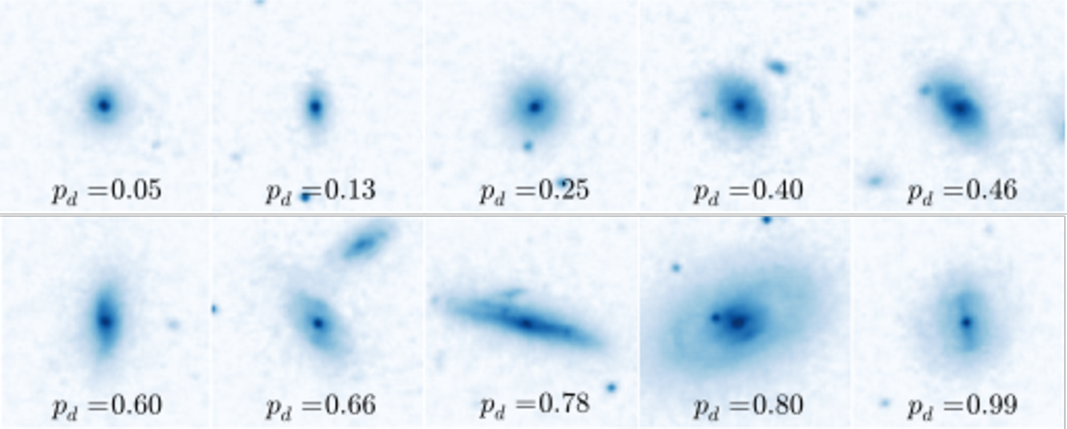
\includegraphics[width=\textwidth]{agn/fig1.pdf}
\caption[SDSS images of galaxies in the \textsc{agn-host} sample]{Randomly selected SDSS \emph{gri} composite images from the sample of $1,244$ Type 2 AGN in a redshift range $0.04 < z < 0.05$.  The galaxies are ordered from least to most featured according to their debiased `disc or featured' vote fraction, $p_d$ (see \citealt{GZ2}). The scale for each image is $0.099~\rm{arcsec/pixel}$.}
\label{mosaic}
\end{figure*}

Since this investigation is focussed on whether an AGN can have an impact on the SF of its host galaxy, possible selection effects must be considered. The extent to which SF could obscure AGN emission was addressed by \cite{schawinski10a}. They showed, via analysis of simulated AGN emission added to star-forming galaxies, that BPT-based selection of AGN produces a complete sample at luminosities of $L[OIII] > 10^{40}~\rm{erg~s}^{-1}$. Above this limit I therefore assume I have selected a complete sample of AGN independent of host galaxy SFR. 

Black hole masses of the \textsc{agn-host} sample are derived from the $M_{BH}-\sigma$ relationship defined in \citet{mcconnell11}:
\begin{equation}
\log_{10}\left(\frac{M_{BH}}{M_{\odot}}\right) = 8.29 + 5.12 ~\log_{10}\left(\frac{\sigma}{200 ~\rm{km} ~s^{-1}}\right). 
\end{equation}
where the velocity dispersion, $\sigma$, is measured from the Balmer lines and is provided in the MPA-JHU catalog \citep{kauffmann03, brinchmann04}. The Eddington ratio, $\lambda_{Edd}$, describes the accretion rate of the black hole and is calculated with the proxy $\lambda_{Edd} = L_{bol}/L_{Edd}$, where $L_{Edd}$ is the Eddington luminosity and $L_{bol}$ is the bolometric luminosity. For obscured (Type 2) AGN the bolometric luminosity cannot be directly measured and so is inferred from the luminosity of the [OIII] emission line, as derived by \citet{heckman04}:
\begin{equation}
\log_{10}L_{bol} = 3.54 + \log_{10}L[OIII]. 
\end{equation}
The Eddington luminosity, $L_{Edd}$, is derived from the black hole mass, $M_{BH}$, as outlined in \citet{binneymerrifield} as:
\begin{equation}
L_{Edd} = 3\times10^4 \left(\frac{M_{BH}}{M_{\odot}}\right) L_{\odot}.
\end{equation}
The distributions of L[OIII], $M_{BH}$ and $\lambda_{Edd}$ of the \textsc{agn-host} sample are shown in Figure~\ref{fig:agndistributions}. SDSS images for 10 randomly selected galaxies from the \textsc{agn-host} sample are shown in Figure~\ref{mosaic}. The decomposition of the \textsc{agn-host} sample into red sequence, green valley and blue cloud galaxies is shown in Tables~\ref{table:agnsubs} and \ref{table:agnqsubs} along with further division by galaxy type and SFR (where available for the \textsc{agn-host} sample from the MPA-JHU catalog) respectively. 


\begin{table}
\caption{Table showing the decomposition of the \textsc{agn-host} sample by galaxy type into the subsets of the colour-magnitude diagram.}
\begin{tabular*}{\textwidth}{l @{\extracolsep{\fill}}cccc}
\hline
\begin{tabular}[c]{@{}c@{}} {\color{white} -} \\ {\color{white} -}  \end{tabular} & All                                                      & Red Sequence                                              & Green Valley                                              & Blue Cloud \\  \hline 
Smooth-like ($p_s > 0.5$)        & \begin{tabular}[c]{@{}c@{}}340\\ (27.3\%)\end{tabular} & \begin{tabular}[c]{@{}c@{}}21\\ (25.0\%)\end{tabular}  & \begin{tabular}[c]{@{}c@{}}105\\ (41.2\%)\end{tabular}   & \begin{tabular}[c]{@{}c@{}}213\\ (23.5\%)\end{tabular}  \\ 
Disc-like ($p_d > 0.5$)          & \begin{tabular}[c]{@{}c@{}}871\\ (70.0\%)\end{tabular} & \begin{tabular}[c]{@{}c@{}}63\\ (75.0\%)\end{tabular}   & \begin{tabular}[c]{@{}c@{}}148\\ (58.0\%)\end{tabular}  & \begin{tabular}[c]{@{}c@{}}660\\ (72.9\%)\end{tabular}  \\
Early-type ($p_s \geq 0.8$) & \begin{tabular}[c]{@{}c@{}}66\\ (5.3\%)\end{tabular}  & \begin{tabular}[c]{@{}c@{}}1\\ (1.2\%)\end{tabular}    & \begin{tabular}[c]{@{}c@{}}14\\ (5.5\%)\end{tabular}    & \begin{tabular}[c]{@{}c@{}}51\\ (5.6\%)\end{tabular}    \\
Late-type ($p_s \geq 0.8$)  & \begin{tabular}[c]{@{}c@{}}569\\ (45.7\%)\end{tabular} & \begin{tabular}[c]{@{}c@{}}39\\ (46.4\%)\end{tabular}    & \begin{tabular}[c]{@{}c@{}}74\\ (29.0\%)\end{tabular}    & \begin{tabular}[c]{@{}c@{}}456\\ (50.4\%)\end{tabular}  \\ \hline
\textbf{Total}                       & \begin{tabular}[c]{@{}c@{}}\textbf{1244} \\ (100.0\%)\end{tabular}                                                & \begin{tabular}[c]{@{}c@{}}84 \\ (6.7\%)\end{tabular} & \begin{tabular}[c]{@{}c@{}}255 \\ (20.5\%)\end{tabular} & \begin{tabular}[c]{@{}c@{}}905 \\ (72.7\%)\end{tabular} \\\hline
\end{tabular*}
\label{table:agnsubs}
\end{table}


\begin{table}
\caption{Table showing the decomposition of the \textsc{agn-host} sample galaxies by their star formation rate in the subsets of the colour-magnitude diagram.}
\begin{tabular*}{\textwidth}{l @{\extracolsep{\fill}}cccc}
\hline
\begin{tabular}[c]{@{}c@{}} {\color{white} -} \\ {\color{white} -}  \end{tabular} 		& All                                                      						& Red Sequence                                              			& Green Valley                                             			 & Blue Cloud \\  \hline 
\begin{tabular}[l]{@{}l@{}}Quenched\\ ($\rm{SFR} < P - 5\sigma$) \end{tabular}				& \begin{tabular}[c]{@{}c@{}}14\\ (1.3\%)\end{tabular} 			& \begin{tabular}[c]{@{}c@{}}9\\ (12.5\%)\end{tabular}    & \begin{tabular}[c]{@{}c@{}}4\\ (1.7\%)\end{tabular}    & \begin{tabular}[c]{@{}c@{}}1\\ (0.1\%)\end{tabular}  \\ 
\begin{tabular}[l]{@{}l@{}}Quenching\\ ($P - 5\sigma < \rm{SFR} < P - \sigma$) \end{tabular}	 & \begin{tabular}[c]{@{}c@{}}335\\ (30.6\%)\end{tabular}			 & \begin{tabular}[c]{@{}c@{}}45\\ (64.3\%)\end{tabular}    & \begin{tabular}[c]{@{}c@{}}139\\ (59.9\%)\end{tabular}    & \begin{tabular}[c]{@{}c@{}}151\\ (19.1\%)\end{tabular}  \\ 
\begin{tabular}[l]{@{}l@{}}Star Forming  \\ ($\rm{SFR} > P -\sigma$) \end{tabular} 			& \begin{tabular}[c]{@{}c@{}}744\\ (68.0\%)\end{tabular} 			& \begin{tabular}[c]{@{}c@{}}16 \\ (22.9\%)\end{tabular}    & \begin{tabular}[c]{@{}c@{}}89\\ (38.4\%)\end{tabular}    & \begin{tabular}[c]{@{}c@{}}639\\ (80.7\%)\end{tabular}  \\ \hline
\textbf{Total}                       														& \begin{tabular}[c]{@{}c@{}}\textbf{1093} \\ (100.0\%)\end{tabular} & \begin{tabular}[c]{@{}c@{}}70 \\ (6.4\%)\end{tabular} & \begin{tabular}[c]{@{}c@{}}232 \\ (21.2\%)\end{tabular} & \begin{tabular}[c]{@{}c@{}}791 \\ (72.4\%)\end{tabular} \\\hline
\end{tabular*}
\label{table:agnqsubs}
\end{table}


\subsection{Defining a control sample}

\begin{figure*}
\centering
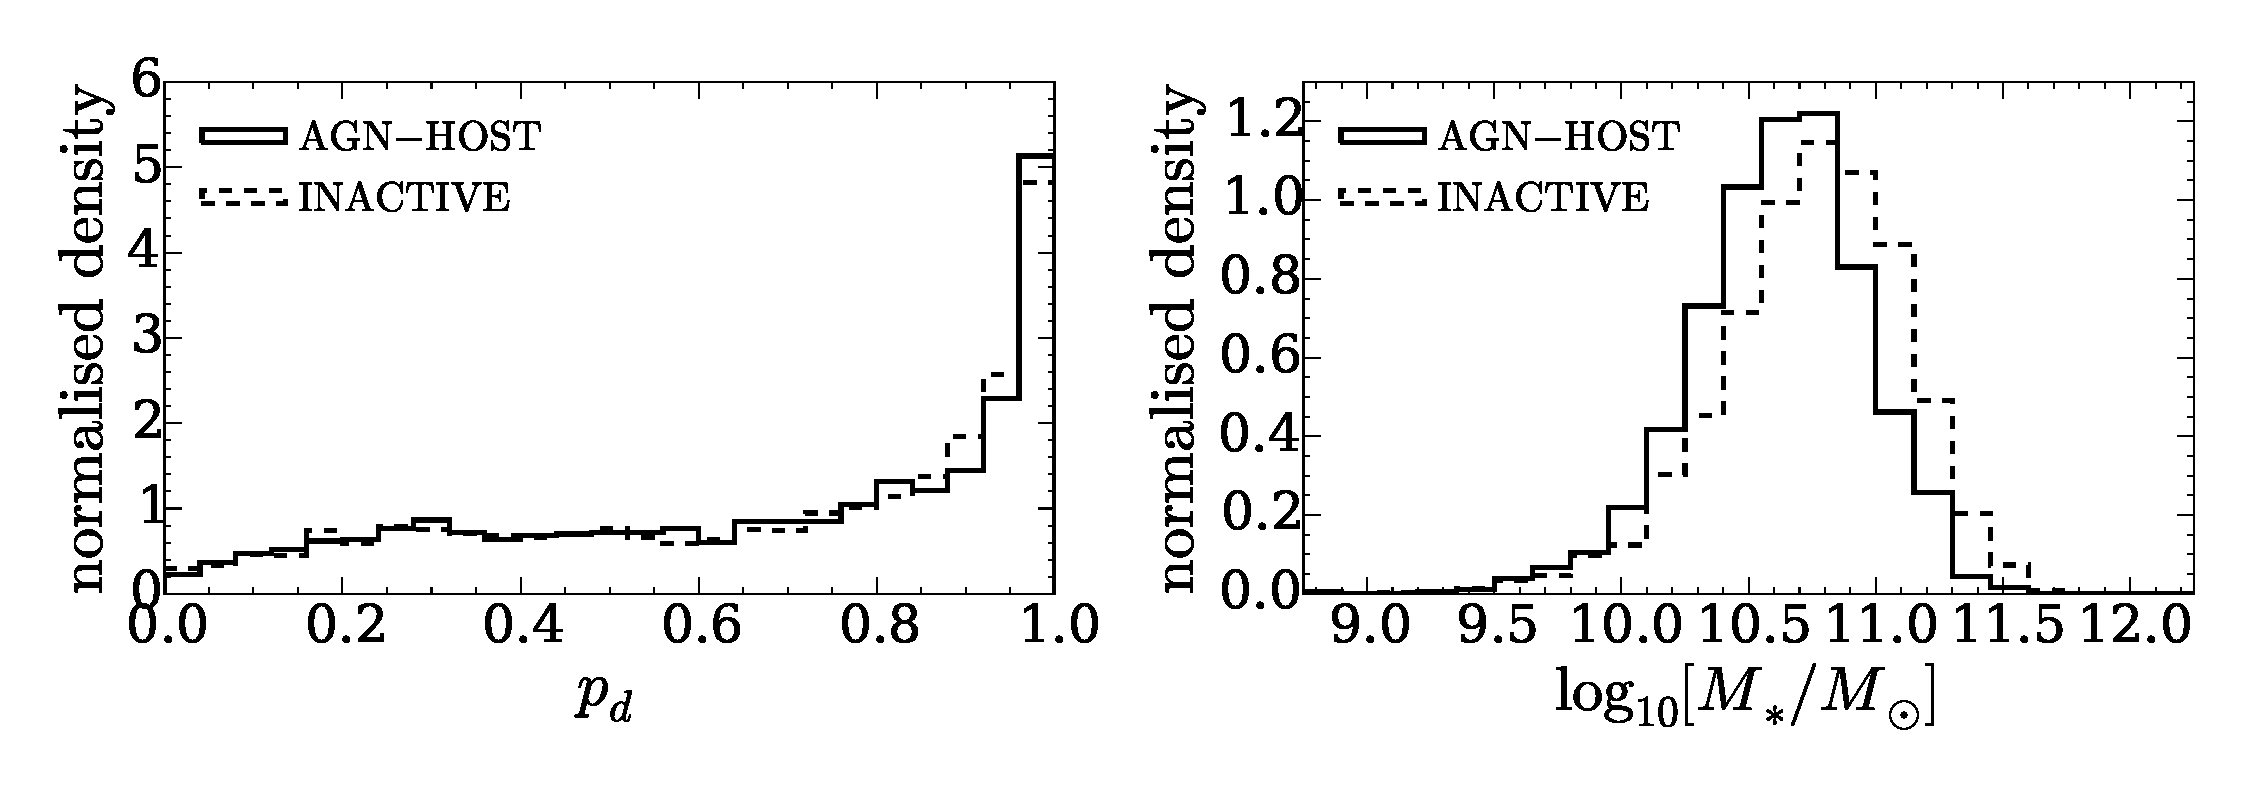
\includegraphics[width=\textwidth]{agn/agn-host_inactive_pd_mass_distributions.pdf}
\caption[Morphology and mass distributions of the \textsc{agn-host} and \textsc{inactive} samples]{Distribution of the GZ2 disc vote fractions ($p_d$; left) and stellar masses (right) in the \textsc{agn-host} sample (solid lines) in comparison to the matched control \textsc{inactive} sample (dashed lines).}
\label{fig:zmdistmatch}
\end{figure*}

\begin{figure}
\centering
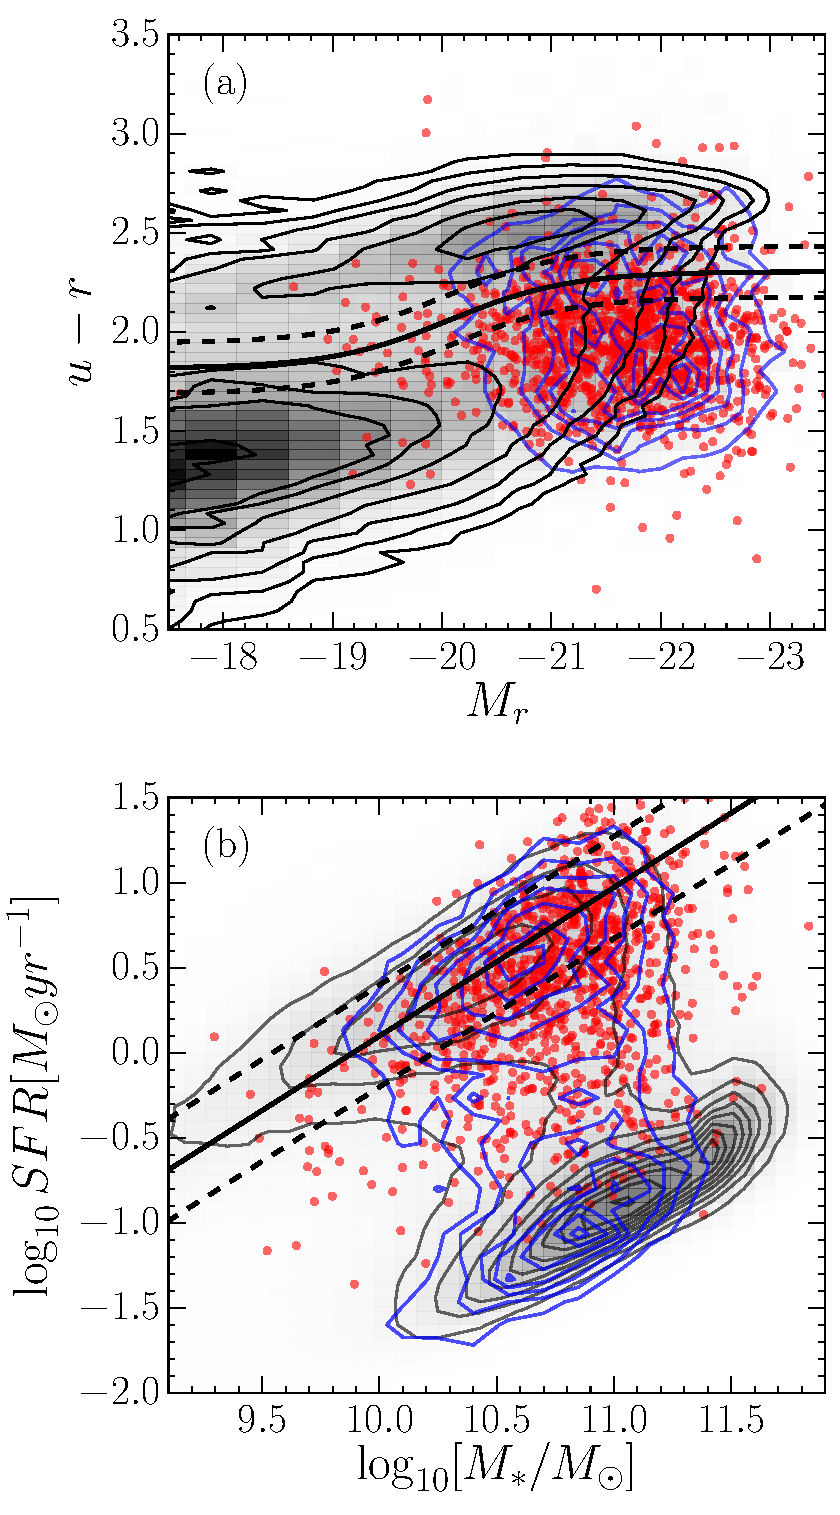
\includegraphics[height=0.75\textheight]{agn/fig3.pdf}
\caption[Colour-magnitude and SFR-mass diagram for \textsc{agn-host} galaxies]{(a) Optical colour-magnitude diagram showing the SDSS DR7 (grey filled contours), the \textsc{agn-host} sample (red circles) and \textsc{inactive} sample (blue contours). The definition of the green valley from \citet{Baldry06} (solid line) with $\pm 1\sigma$ (dashed lines) is shown. (b) SFR-stellar mass diagram showing the MPA-JHU measurements of SFR and $M_*$ of SDSS DR7 galaxies (\citealt{kauffmann03, brinchmann04}; black contours), the \textsc{agn-host} sample (red circles) and \textsc{inactive} sample (blue contours). The star forming `main sequence' from \citet{peng10} is shown by the solid line for $t = 12.8~\rm{Gyr}$, the average observed age of the \textsc{gz2-galex} sample, with $\pm1\sigma$ (dashed lines).}
\label{cmdsfms}
\end{figure}


A control sample of inactive galaxies was constructed by removing from the \textsc{gz2-galex} sample all galaxies with line strengths indicative of potential AGN activity \citep{kauffmann03b}, as well as sources identified as Type 1 AGN by the presence of broad emission lines \citep{Oh15}.  I selected a mass- and morphology-matched inactive sample by identifying between 1 and 5 inactive galaxies for each \textsc{agn-host} galaxy with the same stellar mass (to within $\pm5\%$) and GZ2 `smooth' and `disc' vote fractions (to within $\pm 0.1$) giving $6107$ galaxies. This sample will be referred to as the \textsc{inactive} sample. 


Figure~\ref{fig:zmdistmatch} shows the GZ2 disc vote fraction ($p_d$; left) and stellar mass ($M_*$; right) distributions of the \textsc{agn-host} sample in comparison to the matched \textsc{inactive} sample. A Kolmogorov-Smirnov test revealed the redshift distributions of the \textsc{inactive} and \textsc{agn-host} samples are statistically indistinguishable ($D \sim 0.16$, $p \sim 0.88$). 

The \textsc{agn-host} and \textsc{inactive}  samples are also shown on both an optical colour-magnitude diagram and in the SFR-stellar mass plane in Figure~\ref{cmdsfms} in comparison to the distribution of SDSS DR7 galaxies. SFRs and stellar masses are obtained from the MPA JHU catalog, where available, which follow the prescriptions outlined in \cite{brinchmann04} and \cite{Salim07} for calculating the total aperture corrected galaxy SFR in the presence of an AGN. 

The majority of the \textsc{agn-host} sample would be defined as residing in the blue cloud ($\sim73\%$) on the optical colour-magnitude diagram despite the fact that a significant proportion of the sample ($32\%$) lie more than $1\sigma$ ($0.3$ $\rm{dex}$) below the star forming `main sequence' \citep[][see Figure \ref{cmdsfms} and Table~\ref{table:agnqsubs}]{peng10}.

\subsection{Results}\label{results}

\begin{figure}
\centering{
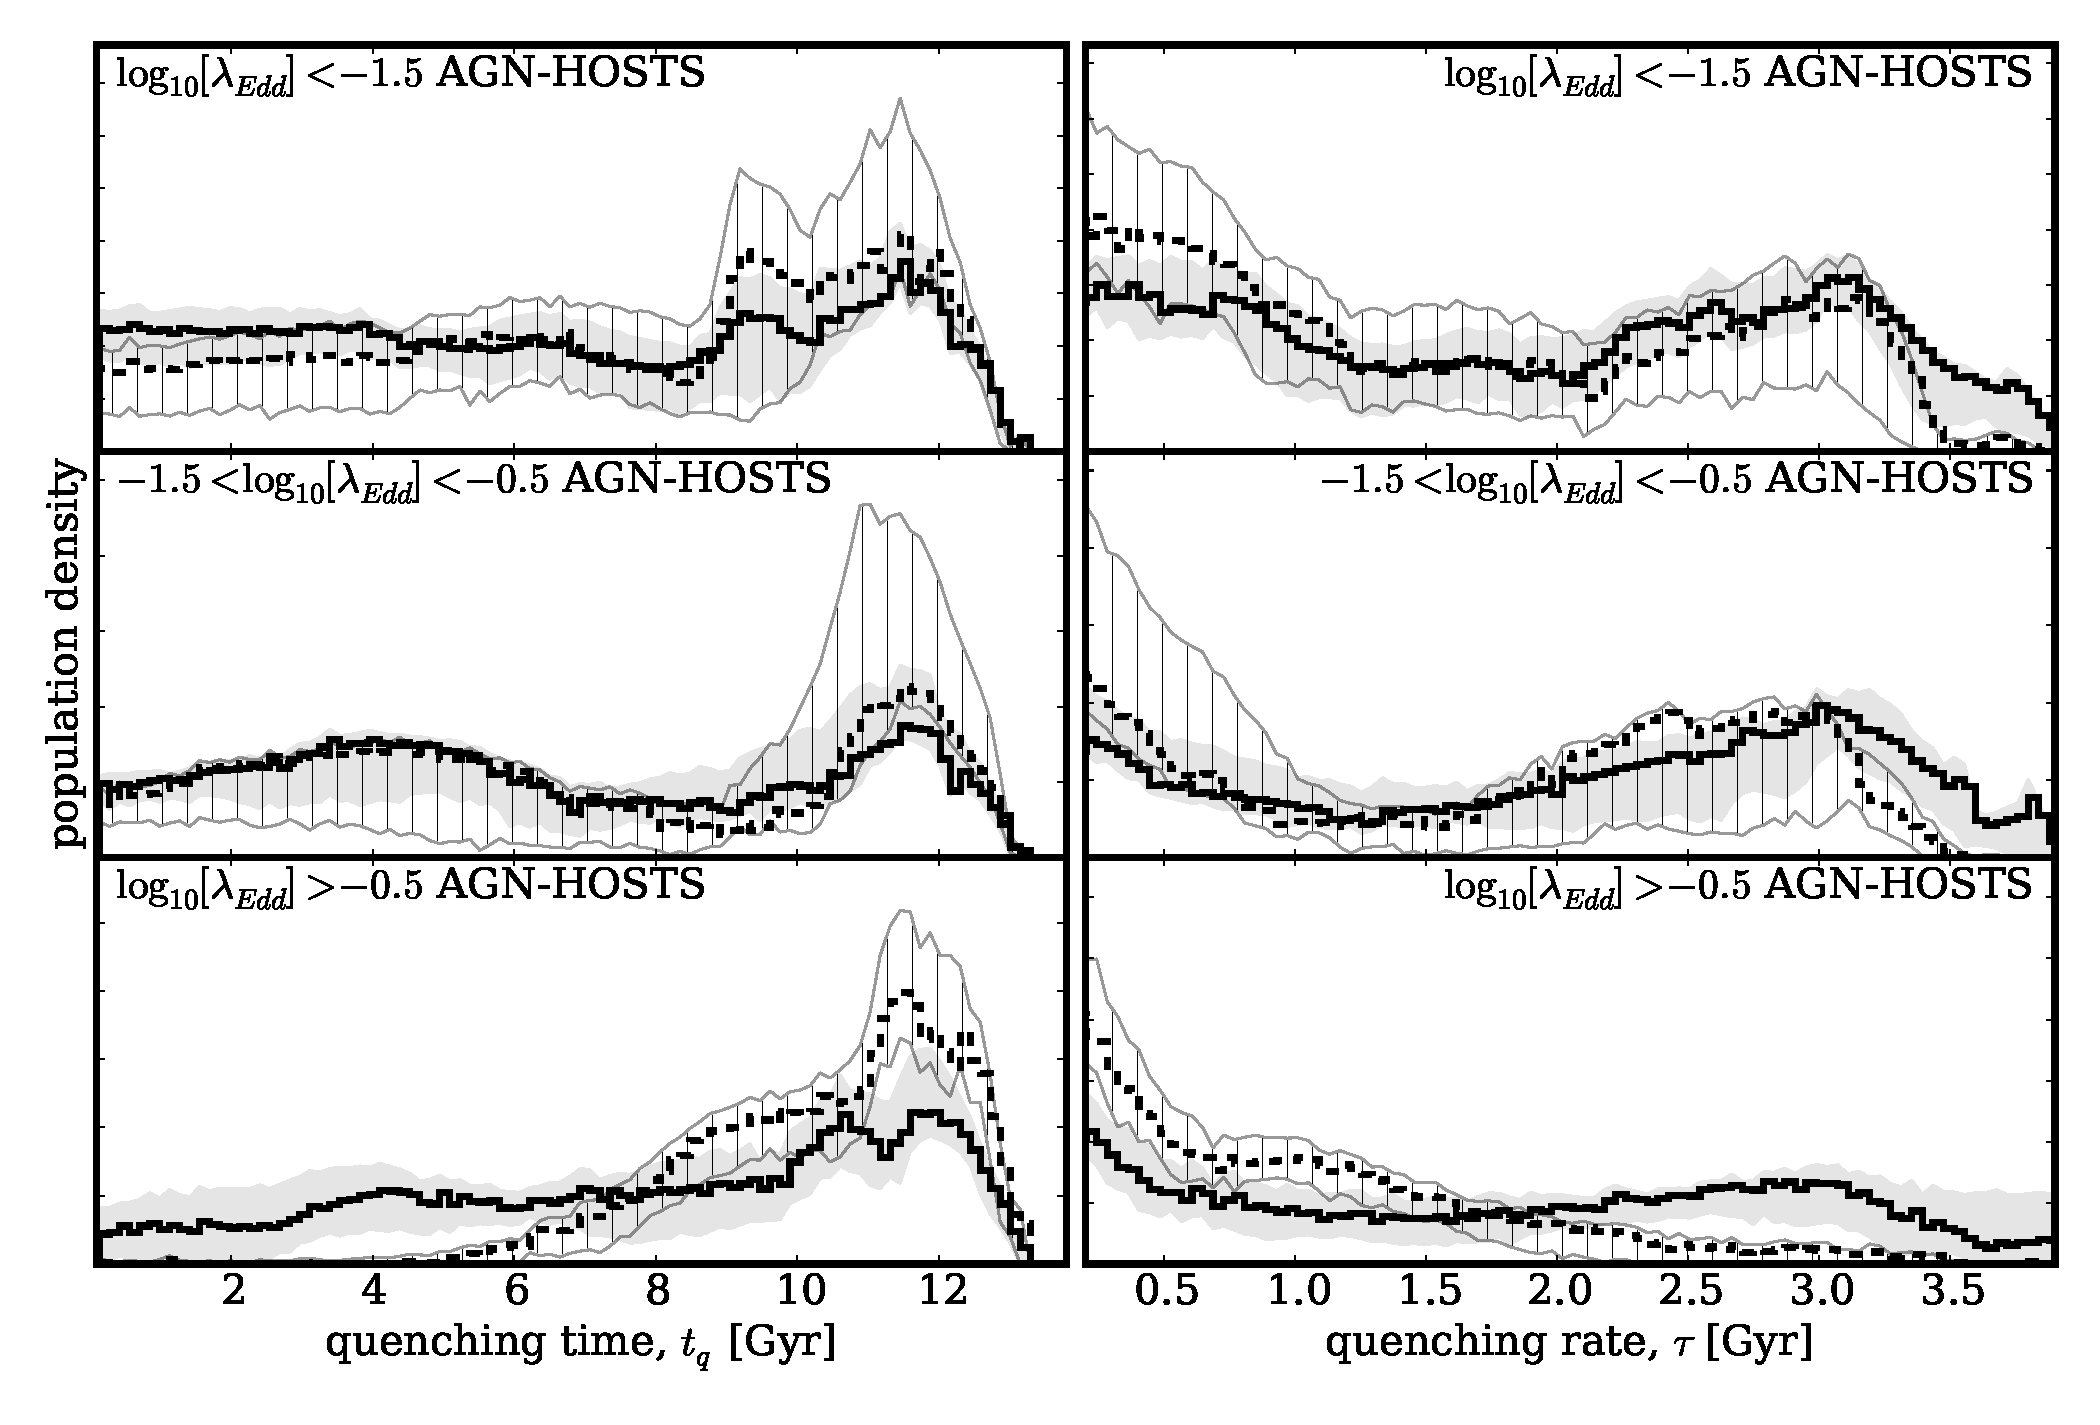
\includegraphics[width=0.92\textwidth]{agn/fig6.pdf}}
\caption[Quenching time and rate population density distributions for the \textsc{agn-host} sample split by Eddington ratio]{Population density distributions for the quenching time ($t_q$; left) and rate ($\tau$; right), normalised so that the areas under the curves are equal. The \textsc{agn-host} sample is split into low (top), medium (middle) and high (bottom) Eddington ratio, $\lambda_{Edd}$, for smooth (dashed) and disc (solid) galaxies. Uncertainties from bootstrapping are shown by the shaded regions for the smooth (grey striped) and disc (grey solid) population densities. A small (large) value of $\tau$ corresponds to a rapid (slow) quench.}
\label{eddratiosplit}
\end{figure}

\begin{figure*}
\centering{
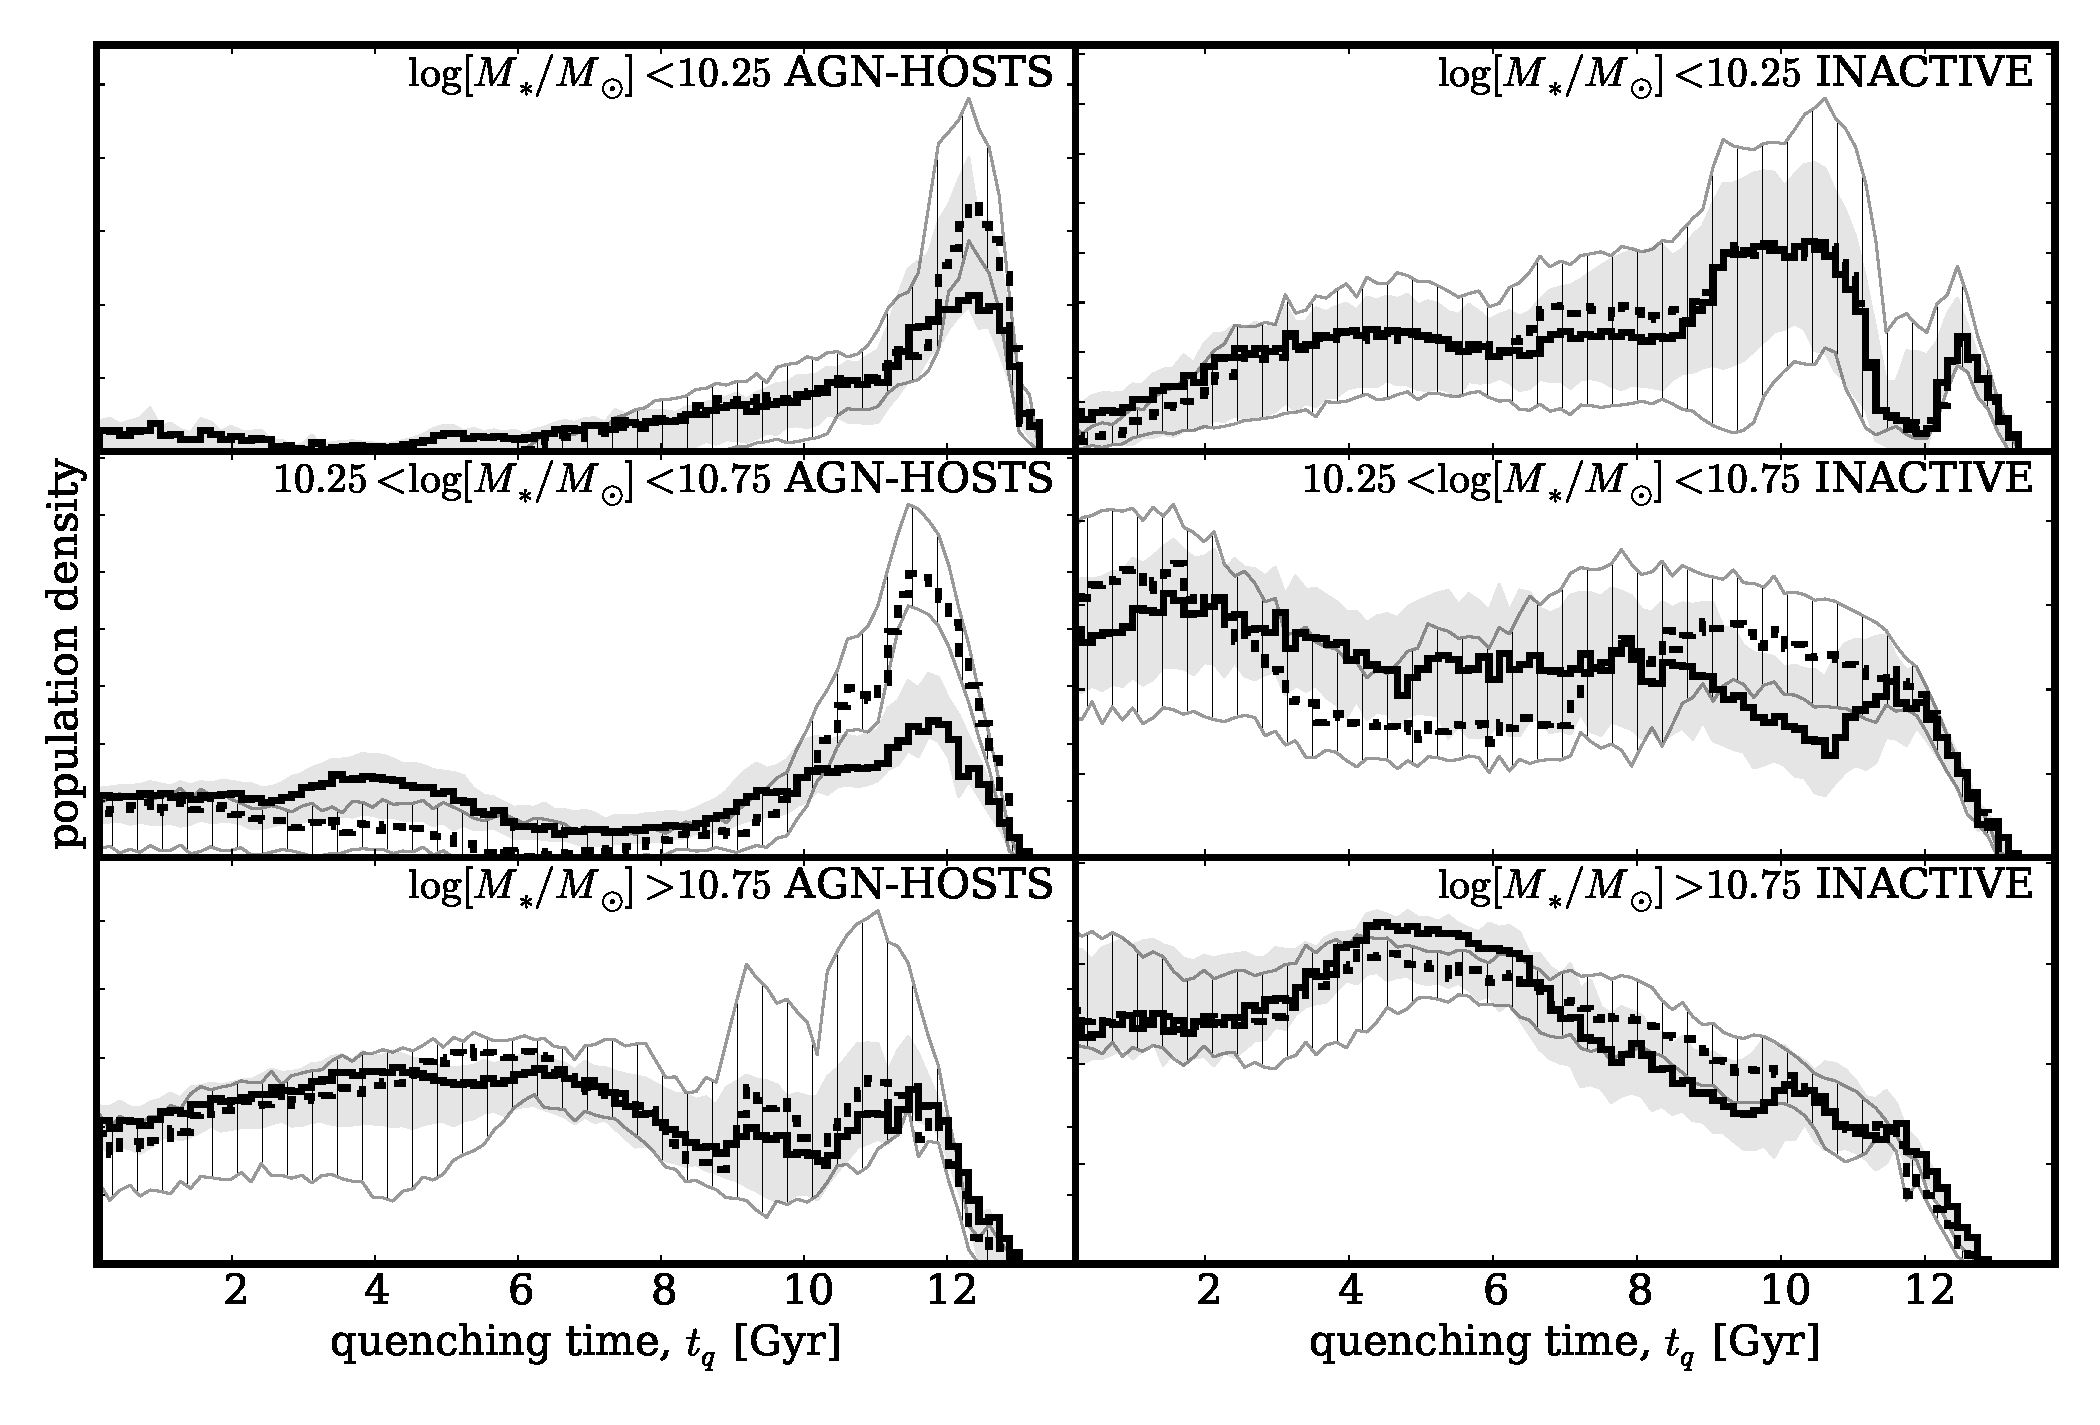
\includegraphics[width=0.92\textwidth]{agn/fig4.pdf}}
\caption[Quenching time population density distributions for the \textsc{agn-host} and \textsc{inactive} samples] {Population density distributions for the quenching time ($t_q$) parameter, normalised so that the areas under the curves are equal. \textsc{agn-host} (left) and \textsc{inactive} (right) galaxies are split into low (top), medium (middle) and high (bottom) mass for smooth (dashed) and disc (solid) galaxies. Uncertainties from bootstrapping are shown by the shaded regions for the smooth (grey striped) and disc (grey solid) population densities. A low (high) value of $t_q$ corresponds to the early (recent) Universe.}
\label{time}
\end{figure*}


\begin{figure*}
\centering{
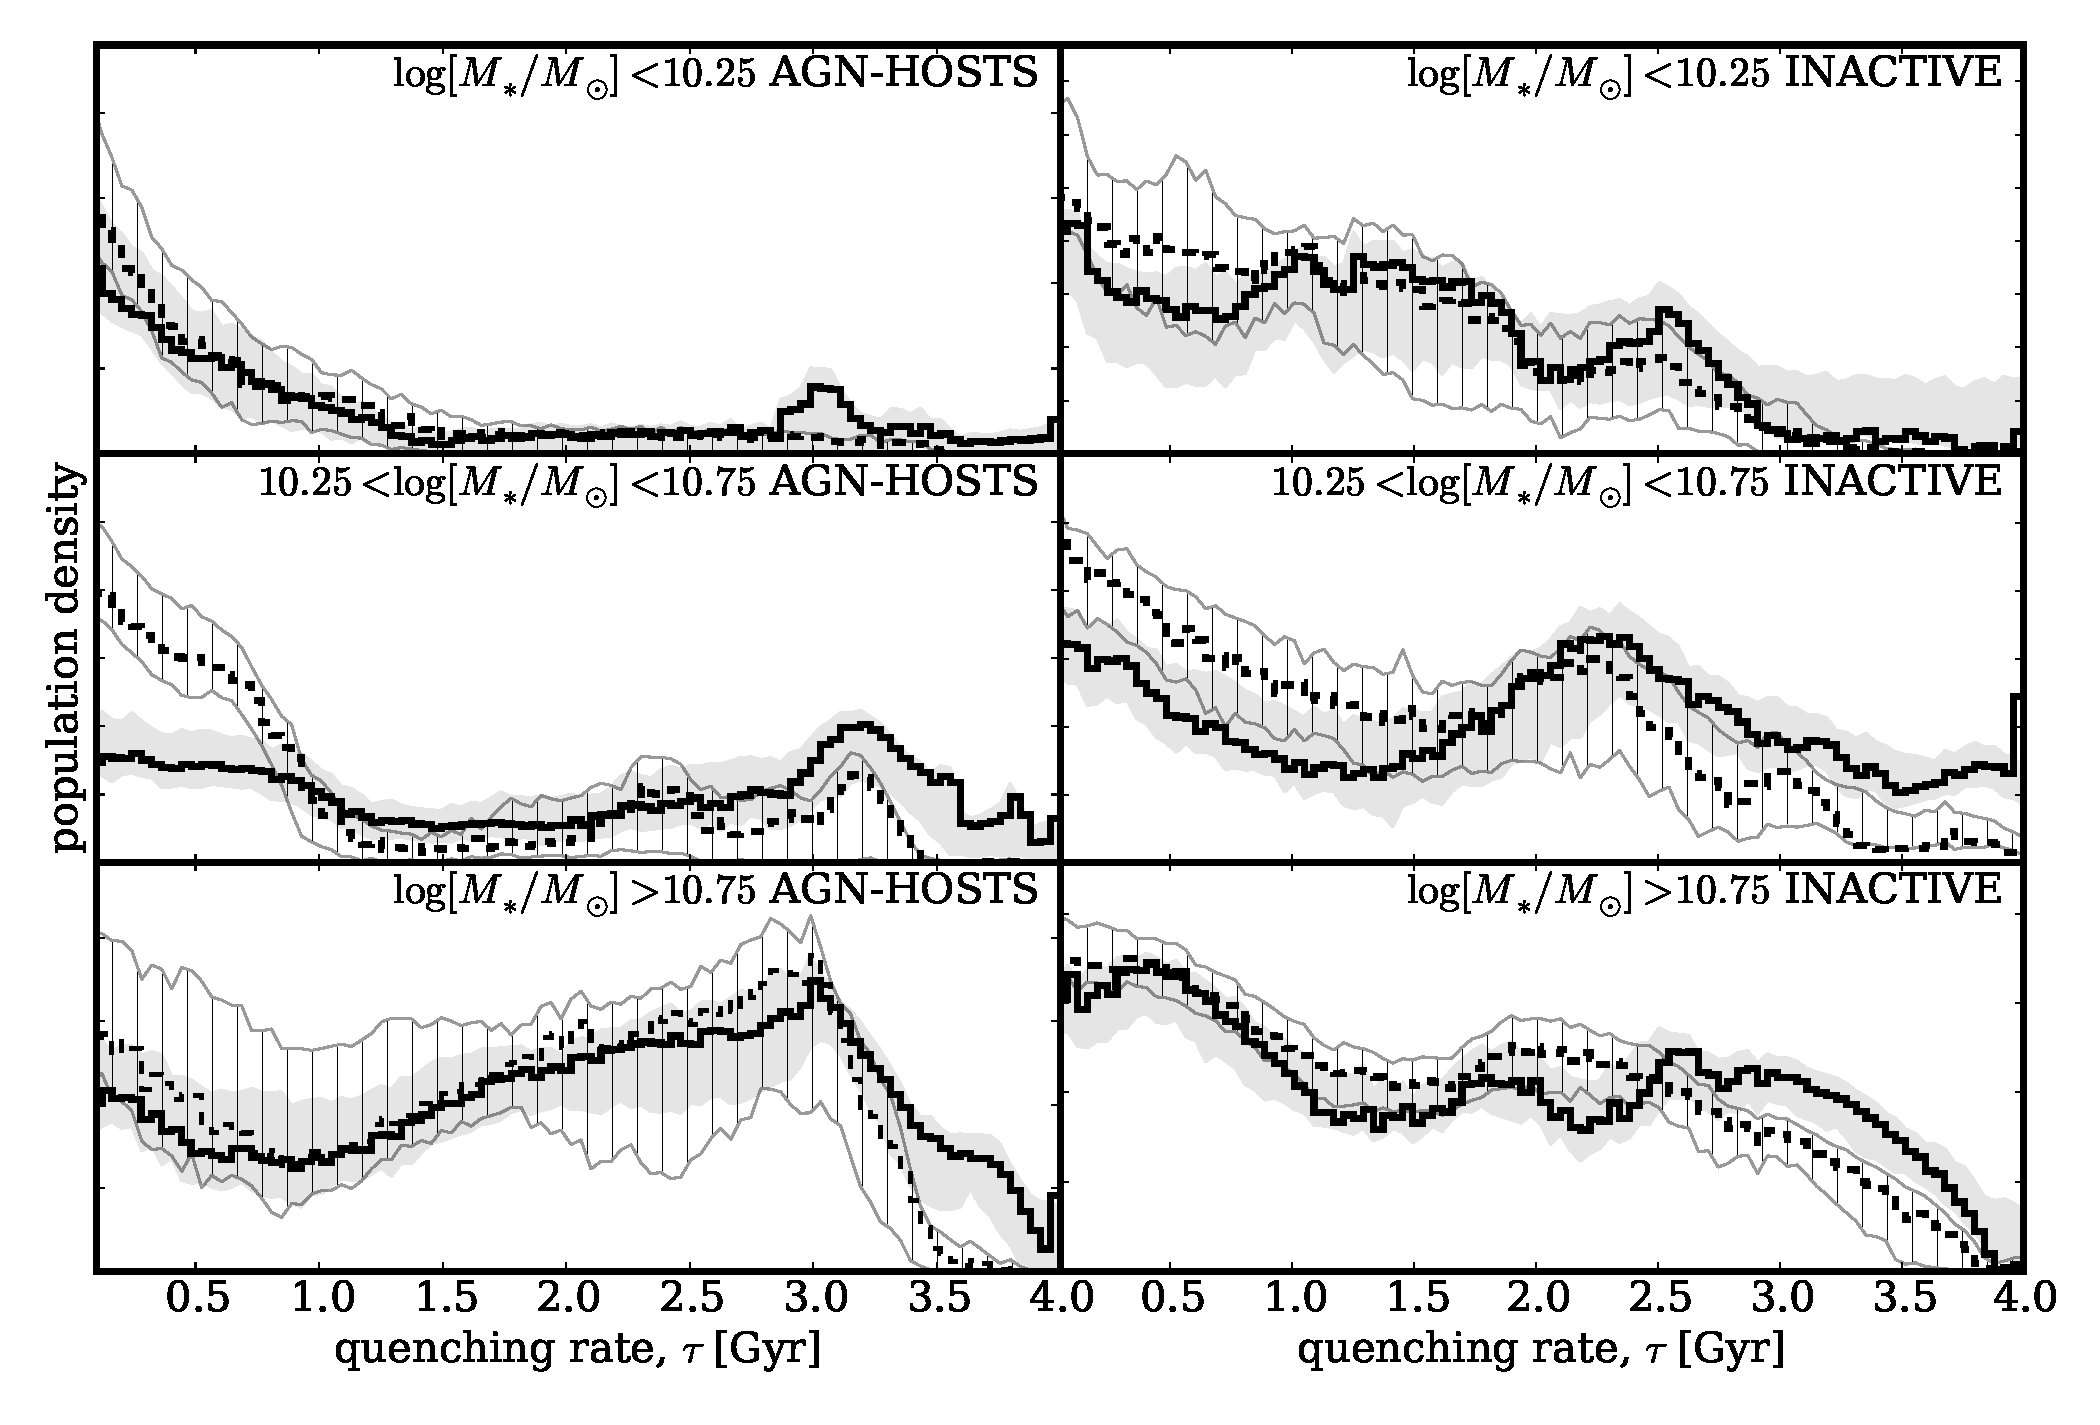
\includegraphics[width=0.92\textwidth]{agn/fig5.pdf}}
\caption[Quenching rate population density distributions for the \textsc{agn-host} and \textsc{inactive} samples]{Population density distributions for the quenching rate ($\tau$), normalised so that the areas under the curves are equal. \textsc{agn-host} (left) host and \textsc{inactive} (right) galaxies are split into low (top), medium (middle) and high (bottom) mass for smooth (dashed) and disc (solid) galaxies. Uncertainties from bootstrapping are shown by the shaded regions for the smooth (grey striped) and disc (grey solid) population densities. A small (large) value of $\tau$ corresponds to a rapid (slow) quench.}
\label{rate}
\end{figure*}


%Figures~\ref{eddratiosplit}, \ref{time} \& \ref{rate} show the population density distributions for the quenching time, $t_q$ and exponential quenching rate, $\tau$, with shaded regions to show the uncertainties for both smooth and disc weighted populations. 

In Figure \ref{eddratiosplit} the \textsc{agn-host} smooth and disc weighted populations are split across three Eddington ratio, $\lambda_{Edd}$, bins to investigate any trends with the accretion rate of the black hole in the population densities for the quenching time and rate. The Eddington ratio boundaries were chosen to give equal numbers of \textsc{agn-host} galaxies in each bin. 

In Figures~\ref{time} \& \ref{rate} the \textsc{agn-host} and \textsc{inactive} smooth and disc weighted populations are split across three mass bins to investigate any trends with mass in the population densities for the quenching time and rate respectively. The mass boundaries were chosen to give roughly equal numbers of inactive galaxies in each bin, before mass matching to the \textsc{agn-host} sample. This decision was made to ensure the mass bins were representative of `typical' galaxies rather than being biased by the mass distribution of the \text{agn-host} sample which tend to occupy higher mass galaxies. 

No cut on the star formation rate is made to the galaxies which contribute to Figures \ref{eddratiosplit}-\ref{rate}, but those galaxies poorly fit by an exponentially declining SFH are down-weighted so that they do not contribute to the results presented here (see Section~\ref{popstarpy} for a description of the \textsc{popstarpy} method). Table~\ref{massbins} contains the percentages of the population densities shown in Figures~\ref{time} \& \ref{rate} in the quenching regimes originally defined in Chapter~\ref{morph} for rapid ($\tau < 1$ Gyr), intermediate ($1 < \tau ~\rm{[Gyr]} < 2$) and slow ($\tau > 2$ Gyr) quenching rates in each of the three mass bins. Uncertainties on the population densities (shown by the shaded regions) are determined from the maximum and minimum values spanned by $N = 1000$ bootstrap iterations, each sampling $90\%$ of the galaxy population. $1\sigma$ uncertainties are quoted for the percentages in Table~\ref{massbins}, calculated from the bootstrapped distributions.


\begin{table*}
{\tiny
\centering{
\caption{Table showing the number of galaxies in each of the three mass bins for both the \textsc{agn-hosts} and \textsc{inactive} galaxy samples and the percentage of the distribution across each morphologically weighted population found in the rapid, intermediate and slow quenching regimes.}
\label{massbins}
\begin{tabular}{c|c|c|c|c|c|c}
\hline
\textsc{sample}                     & \textsc{mass bin}                                        & \textsc{weighting}                  & $\tau < 1 ~\rm{[Gyr]}$                             & $1 < \tau ~\rm{[Gyr]} < 2 $          & $\tau > 2 ~\rm{[Gyr]}$                               & \textsc{number}                                        \\ \hline \hline
\multirow{6}{*}{AGN-HOSTS} & \multirow{2}{*}{$\log [M_*/M_{\odot}] < 10.25 $}                       & $p_d$     & $60\pm_{5}^{23}$                    & $13\pm_{9}^{9}$                    & $28\pm_{19}^{6}$       & \multirow{2}{*}{$165 (13.3\%)$}                      \\
                           &                                                 & $p_s$     & $69\pm_{6}^{14}$                    & $17\pm_{14}^{6}$                   & $14\pm_{7}^{3}$        &                                                      \\ \cline{2-7} 
                           & \multirow{2}{*}{$10.25 < \log [M_*/M_{\odot}] < 10.75$}                    & $p_d$     & $33\pm_{5}^{3}$                     & $15\pm_{4}^{4}$                    & $51\pm_{7}^{4}$        & \multirow{2}{*}{$630 (50.6\%)$}                      \\
                           &                                                 & $p_s$     & $69\pm_{5}^{4}$                     & $7\pm_{4}^{4}$                     & $26\pm_{9}^{5}$        &                                                      \\ \cline{2-7} 
                           & \multirow{2}{*}{$\log [M_*/M_{\odot}] > 10.75$}                      & $p_d$     & $20\pm_{4}^{5}$ & $25\pm_{5}^{7}$                    & $56\pm_{12}^{8}$       & \multirow{2}{*}{$449 (36.1\%)$}                      \\
                           &                                                 & $p_s$     & $24\pm_{3}^{4}$                     & $26\pm_{6}^{5}$                    & $50\pm_{7}^{7}$        &                                                      \\ \hline \hline
\multirow{6}{*}{INACTIVE}  & \multirow{2}{*}{$\log [M_*/M_{\odot}] < 10.25 $}                       & $p_d$     & $37\pm_{14}^{8}$                    & $39\pm_{6}^{8}$                    & $24\pm_{6}^{8}$        & \multirow{2}{*}{$807 (13.2\%)$}                      \\
                           &                                                 & $p_s$     & $47\pm_{11}^{5}$                    & $36\pm_{5}^{9}$                    & $17\pm_{5}^{4}$        &                                                      \\ \cline{2-7} 
                           & \multirow{2}{*}{$10.25 < \log [M_*/M_{\odot}] < 10.75$}                    & $p_d$     &          $30\pm_{3}^{4}$                          &       $18\pm_{3}^{2}$                            &    $51\pm_{4}^{4}$                   & \multirow{2}{*}{$3094 (50.7\%)$}                     \\
                           &                                                 & $p_s$     & $42\pm_{2}^{2}$            & $29\pm_{3}^{3}$   & $30\pm_{4}^{3}$ &                                                      \\ \cline{2-7} 
                           & {\multirow{2}{*}{$\log [M_*/M_{\odot}] > 10.75$}} & $p_d$     & $36\pm_{3}^{3}$            & $24\pm_{4}^{3}$         & $41\pm_{3}^{4}$ & \multicolumn{1}{l}{\multirow{2}{*}{$2206 (36.1\%)$}} \\
                           & \multicolumn{1}{l|}{}                           & $p_s$      & $38\pm_{2}^{2}$              & $28\pm_{4}^{3}$            & $34\pm_{3}^{3}$ & \multicolumn{1}{l}{}                                 \\ \hline                       
\end{tabular}}}
\end{table*}

At all masses, the population density for galaxies within the \textsc{agn-host} population across the quenching time, $t_q$ (left panels of Figure~\ref{time}), is different from that of the inactive galaxies (right panels of Figure~\ref{time}). Recent quenching ($t > 11$ Gyr) is the dominant history for low and medium mass \textsc{agn-host} galaxies, particularly for the smooth weighted population hosting an AGN (solid lines, left panels Figure~\ref{time}). However, this effect is less dominant in higher mass galaxies where quenching at earlier times also has high density (bottom left panel of Figure \ref{time}).


The population densities for the quenching rate, $\tau$, in Figure~\ref{rate} and Table~\ref{massbins} show the dominance of rapid quenching ($\tau < 1$ Gyr) within the \textsc{agn-host} population, particularly for smooth galaxies (solid lines, left panels Figure~\ref{rate}). With increasing mass the dominant quenching rate becomes slow ($\tau > 2$ Gyr). Similar trends in the population density are observed for the \textsc{inactive} population (right panels Figure~\ref{rate}) but the overall distribution is very different. 

In Figure~\ref{eddratiosplit} there is no \textsc{inactive} control sample to act as a comparison, since an Eddington ratio cannot be measured for a black hole that is not accreting. The population densities for the \textsc{agn-host} samples however, show the dominance of rapid and recent quenching as the Eddington ratio increases (i.e. higher black hole accretion rates). A bimodal distribution can be seen for the low Eddington ratio \textsc{agn-host} population (top right panel of Figure~\ref{eddratiosplit}) between both rapid and slow quenching rates. 

The population densities for the \textsc{agn-host} galaxies therefore all show evidence for the dominance of rapid, recent quenching. This result implies the importance of AGN feedback for the evolution within this population.

\subsection{Discussion}\label{sec:agndis}

The differences between the population density distributions of the \textsc{agn-host} and \textsc{inactive} populations in Figures~\ref{time} \& \ref{rate} reveal that an AGN can have a significant effect on the SFH of its host galaxy. Both recent, rapid quenching and early, slow quenching are observed in the population densities of the \textsc{agn-host} population. 

There are however minimal differences between the smooth and disc weighted distributions of the quenching parameters within the \textsc{agn-host} population (comparing solid and dashed lines in the left panels of Figures~\ref{eddratiosplit} - \ref{rate}). This is agreement with the conclusions of \citet{kauffmann03b} who found that the structural properties of AGN hosts depend very little on AGN power. Quenching caused by AGN feedback is therefore morphologically independent; this is unlike the mechanisms discussed in Chapter~\ref{morph}.

Quenching at early times is observed within the \textsc{inactive} population (see right panels of Figure~\ref{time}), where the population density is roughly constant until recent times where the distribution drops off.  This drop-off occurs at earlier times with increasing mass, with a significant lack of quenching occurring at early times for low mass \textsc{inactive} galaxies (top right panel Figure~\ref{time}). This is evidence of downsizing within the \textsc{inactive} galaxy population whereby stars in massive galaxies form first and quench early \citep{Cowie96, Thomas10}. 

The population densities for smooth weighted higher mass (bottom left panels Figures~\ref{time} \& \ref{rate}) and lower Eddington ratio (top panels Figure \ref{eddratiosplit}) \textsc{agn-host} galaxies are also dominated by slow, early quenching. This implies that AGN feedback is not responsible for the cessation of star formation within a proportion of these galaxies, as this quenching has occurred prior to the triggering of the current AGN. I speculate that this is also due to the effects of downsizing rather than being caused by the current AGN. Since the lower Eddington ratio \textsc{agn-host} population is also dominated by this early quenching at slow rates (top panels Figure~\ref{eddratiosplit}) this supports the idea that the AGN is not strong enough to be the cause of this quenching.  This earlier evolution would first form a slowly `dying' or `dead' galaxy typical of massive elliptical galaxies which could then have a recent infall of gas either through a minor merger, galaxy interaction or environmental change, triggering further star formation and feeding the central black hole, triggering an AGN \citep{kaviraj14b}. In turn this AGN can then quench the recent boost in star formation. This track is similar to the evolution history proposed for blue ellipticals \citep[][and detected in the top panel of Figure~\ref{blue_c}]{Kaviraj13, McIntosh14, Haines15}. This SFH would then give rise to the distribution seen within the high mass smooth weighted \textsc{agn-host} population for both time and rate parameters (bottom panels of Figures~\ref{time} \& \ref{rate}).

Alternatively in the high mass disc weighted \textsc{agn-host} population, in which slow, early quenching is also observed (dashed lines bottom left panels of Figures~\ref{time} \& \ref{rate}) this evolution could be due to initially isolated discs evolving slowly by the Kennicutt-Schmidt \citep{schmidt59, kennicutt97} law which can then undergo an interaction or merger to reinvigorate star formation, feed the central black hole and trigger an AGN \citep{Varela04, emsellem15}. These galaxies would need a large enough gas reservoir to fuel both SF throughout their lifetimes and the recent AGN. These high mass galaxies also play host to the most luminous AGN (mean $\log (L[OIII] ~[\rm{erg}~s^{-1}]) \sim 41.6$) and so this SFH challenges the typical merger driven co-evolution of luminous black holes and their host galaxies (see Section~\ref{intbulgeless} for an investigation into an alternative merger free black hole-galaxy co-evolution). 

These recently triggered, low accretion rate AGN in both massive disc and smooth galaxies do not have have the ability to impact the SF across the entirety of a high mass galaxy in a deep gravitational potential \citep{ishibashi12, Zinn13}. This leads to the lower peak for recent, rapid quenching within the high mass, low Eddington ratio \textsc{agn-host} population for both morphologies (left bottom panels of Figures~\ref{time} \& \ref{rate} and top panels of Figure~\ref{eddratiosplit}). 

Conversely, rapid quenching, possibly caused by the AGN itself through negative feedback, is the most dominant history within the low mass (left top panel Figure~\ref{rate}) and high Eddington ratio (bottom left panel of Figure~\ref{eddratiosplit}) \textsc{agn-host} population. Within the medium mass \textsc{agn-host} population a bimodal distribution between these two quenching histories is seen (left middle panel Figure~\ref{rate}), highlighting the strength of this method which is capable of detecting such variation in the SFHs within a population of galaxies. These lower and medium mass galaxies have lower gravitational potentials from which gas may be more readily expelled or heated \citep{tortora09} by jets launched by the strongly accreting AGN. 

\cite{tortora09} model the effects of this jet-induced AGN feedback on a typical early-type galaxy and observe a drastic suppression of star formation on a timescale of $\sim 3 ~\rm{Myr}$. Comparing their synthetic colours with observed colours of SDSS elliptical galaxies, they find the time between the current galaxy age, $t_\mathrm{gal}$ and the time that the feedback began, $t_\mathrm{AGN}$, peaks at $t_\mathrm{gal} - t_\mathrm{AGN} \sim 0.85 ~\rm{Gyr}$. In the top panel of Figure~\ref{time}, the population density for low mass \textsc{agn-host} galaxies has a difference between the peak of the distribution and the average age of the population (galaxy age is calculated as the age of the Universe at the observed redshift, by assuming all galaxies form at $t=0$) of $\sim0.83 ~\rm{Gyr}$. This is in agreement with the timescales for AGN feedback driven quenching derived in the simulations by \citet{tortora09}. This implies that this SFH dominated by recent quenching is \emph{caused} directly by negative AGN feedback.

Rapid quenching is particularly dominant for low-to-medium mass smooth galaxies as seen in the level panels of Figure~\ref{rate}. In Chapter~\ref{morph} I discussed how these incredibly rapid quenching rates could be attributed to mergers of galaxies in conjunction with AGN feedback, which are thought to be responsible for creating the most massive smooth galaxies \citep{conselice03b, springel05b, hopkins08b}. This dominance of rapid quenching across the smooth \textsc{agn-host} population (solid lines in left panels of Figure~\ref{rate}) supports this hypothesis that a merger, having caused a morphological transformation to a smooth galaxy, can also trigger an AGN, causing feedback and cessation of star formation (\citealt{Sanders88, pontzen16}).

Simulations by \cite{sparre16} show that major merger remnants are only quenched when the prescription used for AGN feedback in the model is stronger than their initial fiducial level. They increase the strength of their AGN feedback by decreasing the metallicity, $Z$, of the gas accreted by the black hole; this impacts on the cooling function of the gas $\Lambda(T, Z)$ \citep[see Section 2.1 of][]{sparre16}. This suggest that AGN feedback will therefore have a larger effect on galaxies with lower metallicity. Considering the mass-metallicity relation \citep{tremonti04}, it follows from this argument that AGN feedback will have a greater effect on galaxies with lower mass. This provides more support to the hypothesis that the dominance of rapid, recent quenching across the low and medium mass \textsc{agn-host} population (left panels Figures~\ref{time} \& \ref{rate}) is caused directly by the AGN.

 \begin{figure*}
\centering{
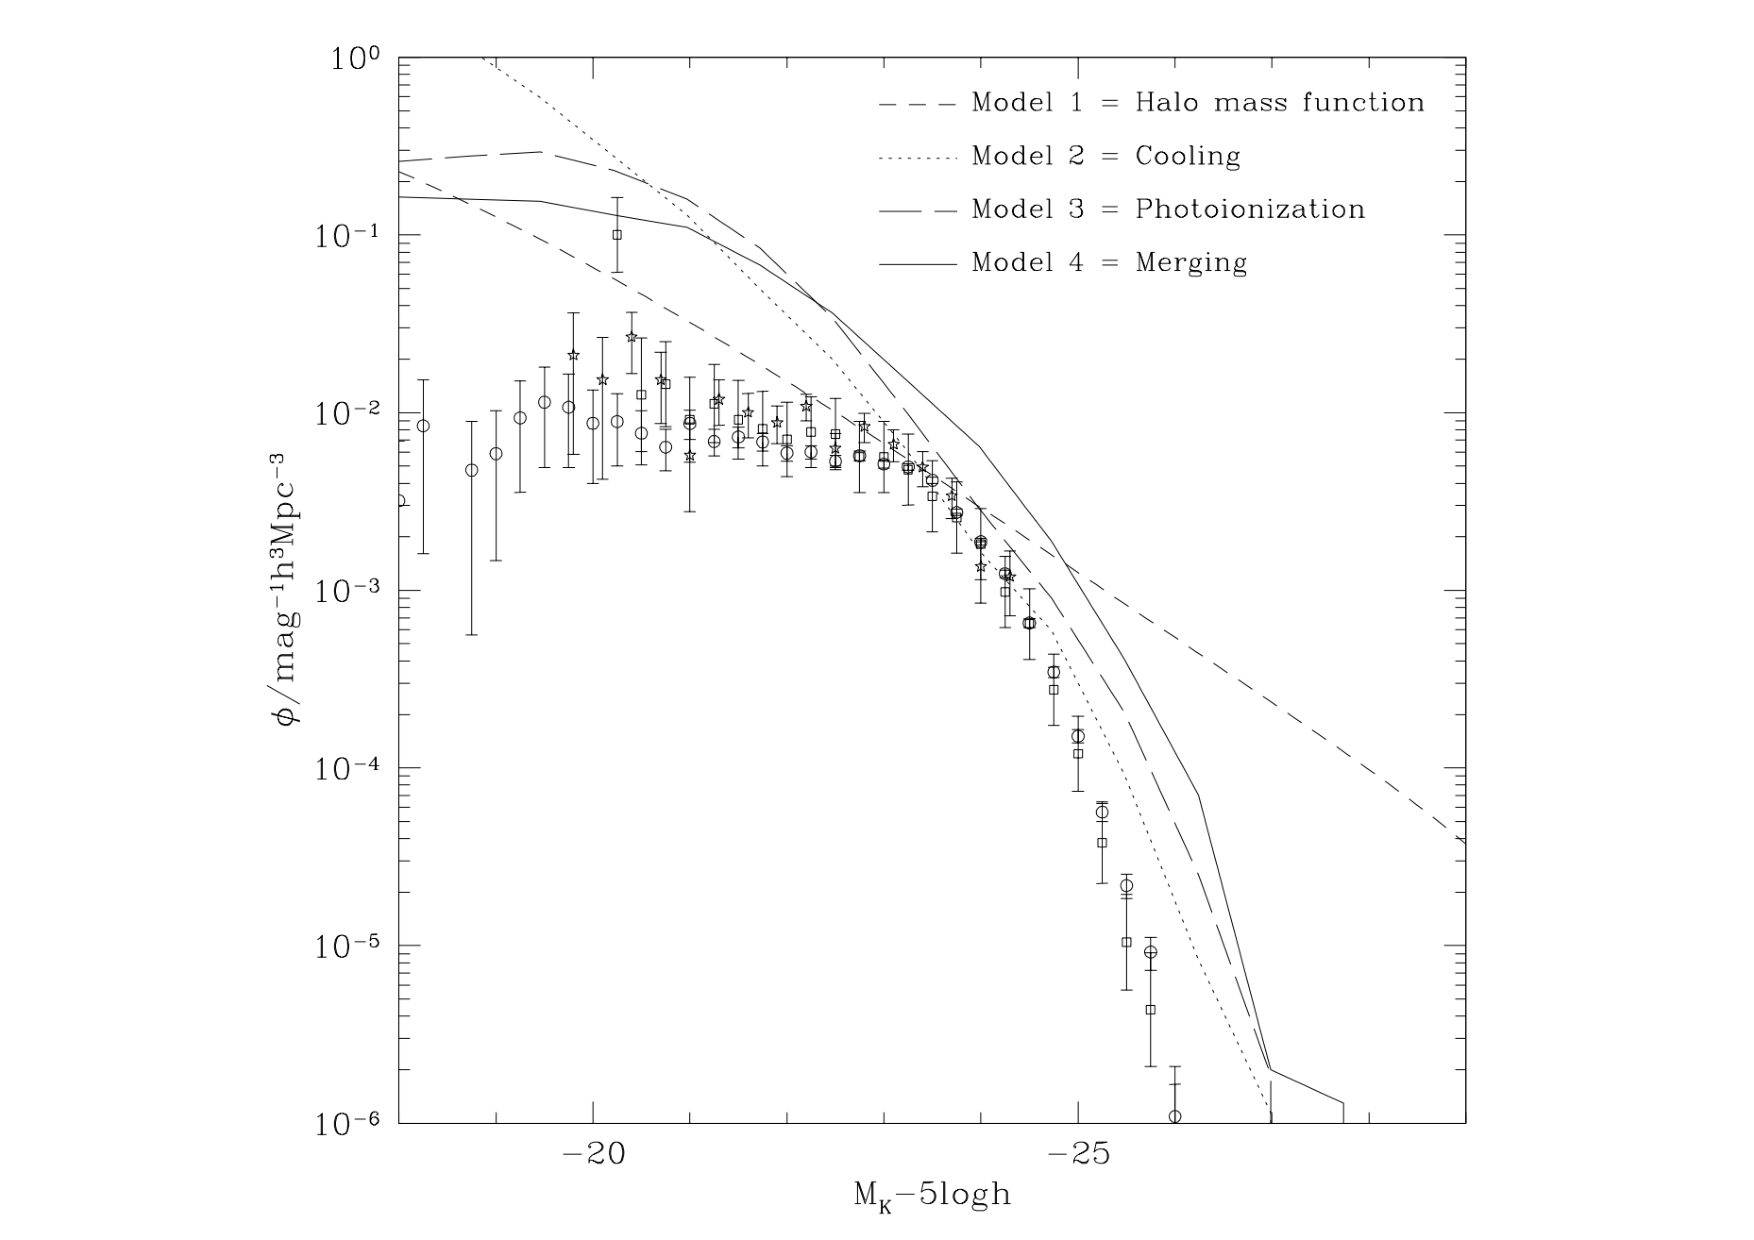
\includegraphics[width=\textwidth]{agn/fig7.pdf}}
\caption[Galaxy luminosity function from observations and simulations: Figure 1 of \cite{benson03}]{Figure 1 from \cite{benson03} showing the K-band luminosity function of galaxies, with $h=0.65$. The points show the observational determinations of \cite[][circles]{cole01}, \cite[][squares]{kochanek01}, and \cite[][$z < 0.1$, stars]{huang03}. Lines show model results investigated by \cite{benson03} to determine what shapes this luminosity function; they concluded that including prescriptions for AGN feedback (supernova feedback winds) can help match the simulations to the data at the bright (faint) end of the luminosity function. The knee of the function occurs at $M_K -5\log_{10} h \sim 23.5$, which is an approximate stellar mass of $\log_{10}[M_*/M_{\odot}] \sim 10.3$, assuming a mass-to-light ratio of $(M/L)_K = 0.8$ \citep{brinchmann00}.}
\label{lumfunc}
\end{figure*}

This mechanism of AGN feedback was originally proposed to regulate the number galaxies at the bright (or high mass) end of the luminosity function in cosmological simulations (see Chapter \ref{intro}). The shape of the observed K-band luminosity function can be seen in Figure~\ref{lumfunc} \citep[Figure 1 from][]{benson03}, falling away from model estimates below a K-band magnitude of $M_K -5\log_{10} h \sim 23.5$, or above an approximate stellar mass of $\log_{10}[M_*/M_{\odot}] \gtrsim 10.3$, assuming a mass-to-light ratio of $(M/L)_K = 0.8$ \citep{brinchmann00}. However, it is the low and medium mass \textsc{agn-host} populations where this rapid recent quenching is dominant (see left panels Figures~\ref{time} \& \ref{rate}). At first this seems contradictory to the arguments posed to constrain the shape of the luminosity function, but with some thought the two results can be reconciled. 

The knee of the luminosity function is the point at which AGN feedback starts to impact the masses of galaxies; this occurs at $\log_{10}[M_*/M_{\odot}] \gtrsim 10.3$, which lies at the lower edge of the medium mass \textsc{agn-host} population studied here. The quenching observed in the low and medium mass \textsc{agn-host} populations will stop the masses of these galaxies from growing any larger in the future. In turn these now quenched galaxies will contribute to dry mergers, which would otherwise have had high gas fractions; limiting the mass of the merger remnants. The combination of these two effects, caused initially by the quench of a lower mass galaxy by negative AGN feedback, will reduce the number of galaxies which will be able to grow to populate the high mass end of the luminosity function. 

However, there still remains the possibility that the AGN is not the cause of the quenching observed, but merely a \emph{consequence} of an alternative quenching mechanism. This idea is supported by simulations showing that the exhaustion of gas by a merger fuelled starburst could cause such a rapid quench in star formation and in turn also trigger an AGN \citep{Croton06, Wild09, Snyder11, Hayward14}. \citet{Yesuf14} also showed that AGN are more commonly hosted by post starburst galaxies, with the peak AGN activity appearing $\geq 200 \pm 100 ~\rm{Myr}$ after the starburst. Such a SFH is not accounted for in the models presented here (see Section ~\ref{sec:future} for a discussion), however this scenario is still consistent with the results presented in this paper; that AGN which are \emph{currently} active have been detected in host galaxies $\sim 1~\rm{Gyr}$ after the onset of quenching. Solving this issue of \emph{cause} vs. \emph{consequence} will not be possible with the currently available SDSS photometry. The advent of Integral Field Unit (IFU) surveys with many aperture fibres per galaxy per observation (such as the MaNGA \citep{bundy15}, SAMI \citep{croom12} and CALIFA \citep{sanchez12} surveys) will allow this problem to be studied by observing the change in quenching parameters with increasing distance from the galaxy nucleus (see Section \ref{sec:future} for a more detailed discussion). 
 

Not all galaxies in the \textsc{agn-host} and \textsc{inactive} samples are quenching (as seen in Figure \ref{cmdsfms}) with a significant proportion of both the \textsc{agn-host} and \textsc{inactive} samples lying on the star forming `main sequence'. A galaxy can therefore still maintain star formation whilst hosting an AGN. The results presented in Section \ref{results} only reflect the trends for galaxies that have undergone or are currently undergoing quenching within the \textsc{agn-host} population and can therefore be accurately fit by an exponentially declining SFH. This prevalence of star forming AGN host galaxies, combined with the results above allows us to consider that either: (i)  the AGN are the cause of the rapid quenching observed but only in gas-poor host galaxies where they can have a large impact, (ii) the AGN are a consequence of another quenching mechanism but can also be triggered by other means which do not cause quenching, or (iii) the SFR of a galaxy can recover post-quench and return to the star forming sequence after a few Gyr (see recent simulations by \citealt{pontzen16} and \citealt{sparre16}). Further investigation will therefore be required to determine the nature of this quenching (see Section \ref{sec:future} for a discussion of proposed future work).


%%%%%%%%%%%%%%%%%%%%%%%%%%%%%%%%%%%%%%%%%%%%%%%%%%%%%%%%%%%%%%%%%%%%%%%%%
%%%%%%%%%%%%%%%%%%%%%%%%%%%%%%%%%%%%%%%%%%%%%%%%%%%%%%%%%%%%%%%%%%%%%%%%%
%%%%%%%%%%%%%%%%%%%%%%%%%%%%%%%%%%%%%%%%%%%%%%%%%%%%%%%%%%%%%%%%%%%%%%%%%
%%%%%%%%%%%%%%%%%%%%%%%%%%%%%%%%%%%%%%%%%%%%%%%%%%%%%%%%%%%%%%%%%%%%%%%%%
%%%%%%%%%%%%%%%%%%%%%%%%%%%%%%%%%%%%%%%%%%%%%%%%%%%%%%%%%%%%%%%%%%%%%%%%%
%%%%%%%%%%%%%%%%%%%%%%%%%%%%%%%%%%%%%%%%%%%%%%%%%%%%%%%%%%%%%%%%%%%%%%%%%
%%%%%%%%%%%%%%%%%%%%%%%%%%%%%%%%%%%%%%%%%%%%%%%%%%%%%%%%%%%%%%%%%%%%%%%%%
%%%%%%%%%%%%%%%%%%%%%%%%%%%%%%%%%%%%%%%%%%%%%%%%%%%%%%%%%%%%%%%%%%%%%%%%%
%%%%%%%%%%%%%%%%%%%%%%%%%%%%%%%%%%%%%%%%%%%%%%%%%%%%%%%%%%%%%%%%%%%%%%%%%
%%%%%%%%%%%%%%%%%%%%%%%%%%%%%%%%%%%%%%%%%%%%%%%%%%%%%%%%%%%%%%%%%%%%%%%%%
 

\newpage

\section{Bulgeless galaxies hosting growing black holes}\label{sec:intbulgeless}

\emph{The work in the following chapter is in preparation for submission to MNRAS in Simmons, Smethurst \& Lintott (in prep.). I was responsible for the spectral data reduction and statistical analysis and assisted in the interpretation of the results.}

%INSERT PARAGRAPH LEADING ON FROM PREVIOUS SECTION

Although the study of large populations of galaxies provides crucial information to constrain the processes governing galaxy evolution, valuable insight can still be discerned from detailed observations of a smaller sample of rare objects. 

The strong correlations that exist between black hole mass and velocity dispersion \citep{magorrian98, merritt01, hu08, kormendy11a, mcconnell11}, bulge stellar mass \citep{marconi03, haringrix04}, and total stellar mass \citep{cisternas11} suggest that galaxies co-evolve with their central super massive black holes (SMBH). Since mergers can grow both bulges and black holes these correlations have been interpreted as the result of a few mergers within a Hubble time \citep{peng07, hopkins08a, jahnke11}. A growing black hole must accrete matter and is therefore observed as an AGN during this time period. Understanding the triggering mechanisms of AGN which kick-start this process of simultaneous galaxy and black hole evolution and possible subsequent feedback from the AGN, is therefore important. However, in Section \ref{sec:agnfeedback}, I presented the argument that disc galaxies currently hosting an AGN could have started quenching at early times with very slow quenching rates, suggesting an alternative to the typical rapid and violent merger driven galaxy-black hole coevolution scenario \citep{hopkins08a}. 

A secular co-evolution of galaxy and black hole has been proposed by previous works \citep{greene10b, jiang11b, cisternas11, Simmons11,schawinski11, kocevski12} and was investigated by \citet{Simmons13} who studied 13 AGN residing in disc dominated host galaxies, whose accretion histories are assumed to be merger free. In the following work I examine a larger sample of disc galaxies, visually identified as bulgeless or disc dominated, hosting an AGN and investigate the locations of these galaxies on typical galaxy-black hole scaling relations. Since the disc galaxies in this sample will have different dynamical histories to bulge dominated galaxies, their black hole masses are not expected to correlate in the same way to their stellar masses if different dynamical histories lead to different mechanisms for black hole growth. 

%The most famous of these scaling relations is the $M-\sigma$ relation. This is a well studied relationship \citep{magorrian98, merrit01, kormendy01, tremaine01, marconi01, graham07, graham08, greene10, mcconnell11, beifoiri12, mcconnell13} and is hypothesised to arise due to the merger driven co-evolution increasing the mass of the black hole at the same time as increasing the velocity dispersion of the galaxy \citep{peng07, hopkins08a, jahnke11}. The black hole mass has similarly been found to correlate with the stellar mass of the galaxy bulge \citep{marconi03, haringrix04} and the total galaxy stellar mass \citep{cisternas11}.


%%%%%%%%%%%%%%%%%%%%%%%%%%%%%%%%%%%%%%%%%%%%%%
%
%
\subsection{Observational Data}\label{sec:data}
%
%
%%%%%%%%%%%%%%%%%%%%%%%%%%%%%%%%%%%%%%%%%%%%%%

The goal of this study is to investigate black hole growth in galaxies whose growth histories have been dominated by relatively calm, slow processes. A sample of growing (i.e. active) black holes hosted in disc-dominated galaxies is therefore required. Optimally, the AGN should have broad emission lines to facilitate measurement of black hole masses via well-established relations between line flux and width and black hole mass. Previously, \citet{Simmons13} investigated a sample of 13 pure disc galaxies hosting AGN. The selection method used in that study selected against very massive black holes with unobscured emission: only 2 AGN of 13 showed clear signs of broadened line emission in their SDSS spectra, leading to calculated black hole masses of $4 \times 10^6 \mmsun$ and $1 \times 10^7 \mmsun $. Here the aim is to select AGN hosted in disc-dominated galaxies at all masses with broad emission lines that can be used to calculate black hole masses through virial assumptions (see Section~\ref{sec:bhmass}). Below the methods used to select both a disc dominated AGN sample along with a control sample of typical AGN host galaxies are described.

%%%%%%%%%%%%%%%%%%%%%%%%%%%%%%%%%%%%%%%%%%%%%%
\subsubsection{Selecting disc-dominated AGN host galaxies}\label{sec:selectAGN}% including where we get AGN luminosities from
%%%%%%%%%%%%%%%%%%%%%%%%%%%%%%%%%%%%%%%%%%%%%%

Asample of unobscured AGN with broad emission lines must first be selected, so that black hole masses may be measured from well-established correlations between emission line properties, such as the FWHM of the broadened $H\alpha$ emission line, and black hole masses \citep[e.g.,][]{gh07a, jiang11a,xiao11, peterson14}. 

These unobscured AGN have characteristic colours in multi-wavelength imaging, particularly in X-ray, optical and infrared bands \citep{kauffmann03b, dstern05, goulding09, kauffmann09, aird12, mendez13, azadi16, cowley16, harrison16}. Given the existence of all-sky surveys at many of the wavelengths relevant to the selection of unobscured AGN, it is now possible to construct larger samples of sources identified as unobscured AGN with high likelihood.

An initial sample of AGN was selected using the W2R sample of \citet{edelson12}, comprised of $4,316$ sources identified using multi-wavelength data from the \emph{Wide-field Infrared Survey Explorer} \citep[\emph{WISE};][]{wright10}, Two Micron All-Sky Survey \citep[2MASS;][]{skrutskie06}, and \emph{ROSAT} all-sky survey \citep[RASS;][]{voges99}. This multi wavelength photometric, all-sky selection, selects unobscured AGN at $>95$ per cent confidence \citep{edelson12}.


\begin{figure*}
\centering
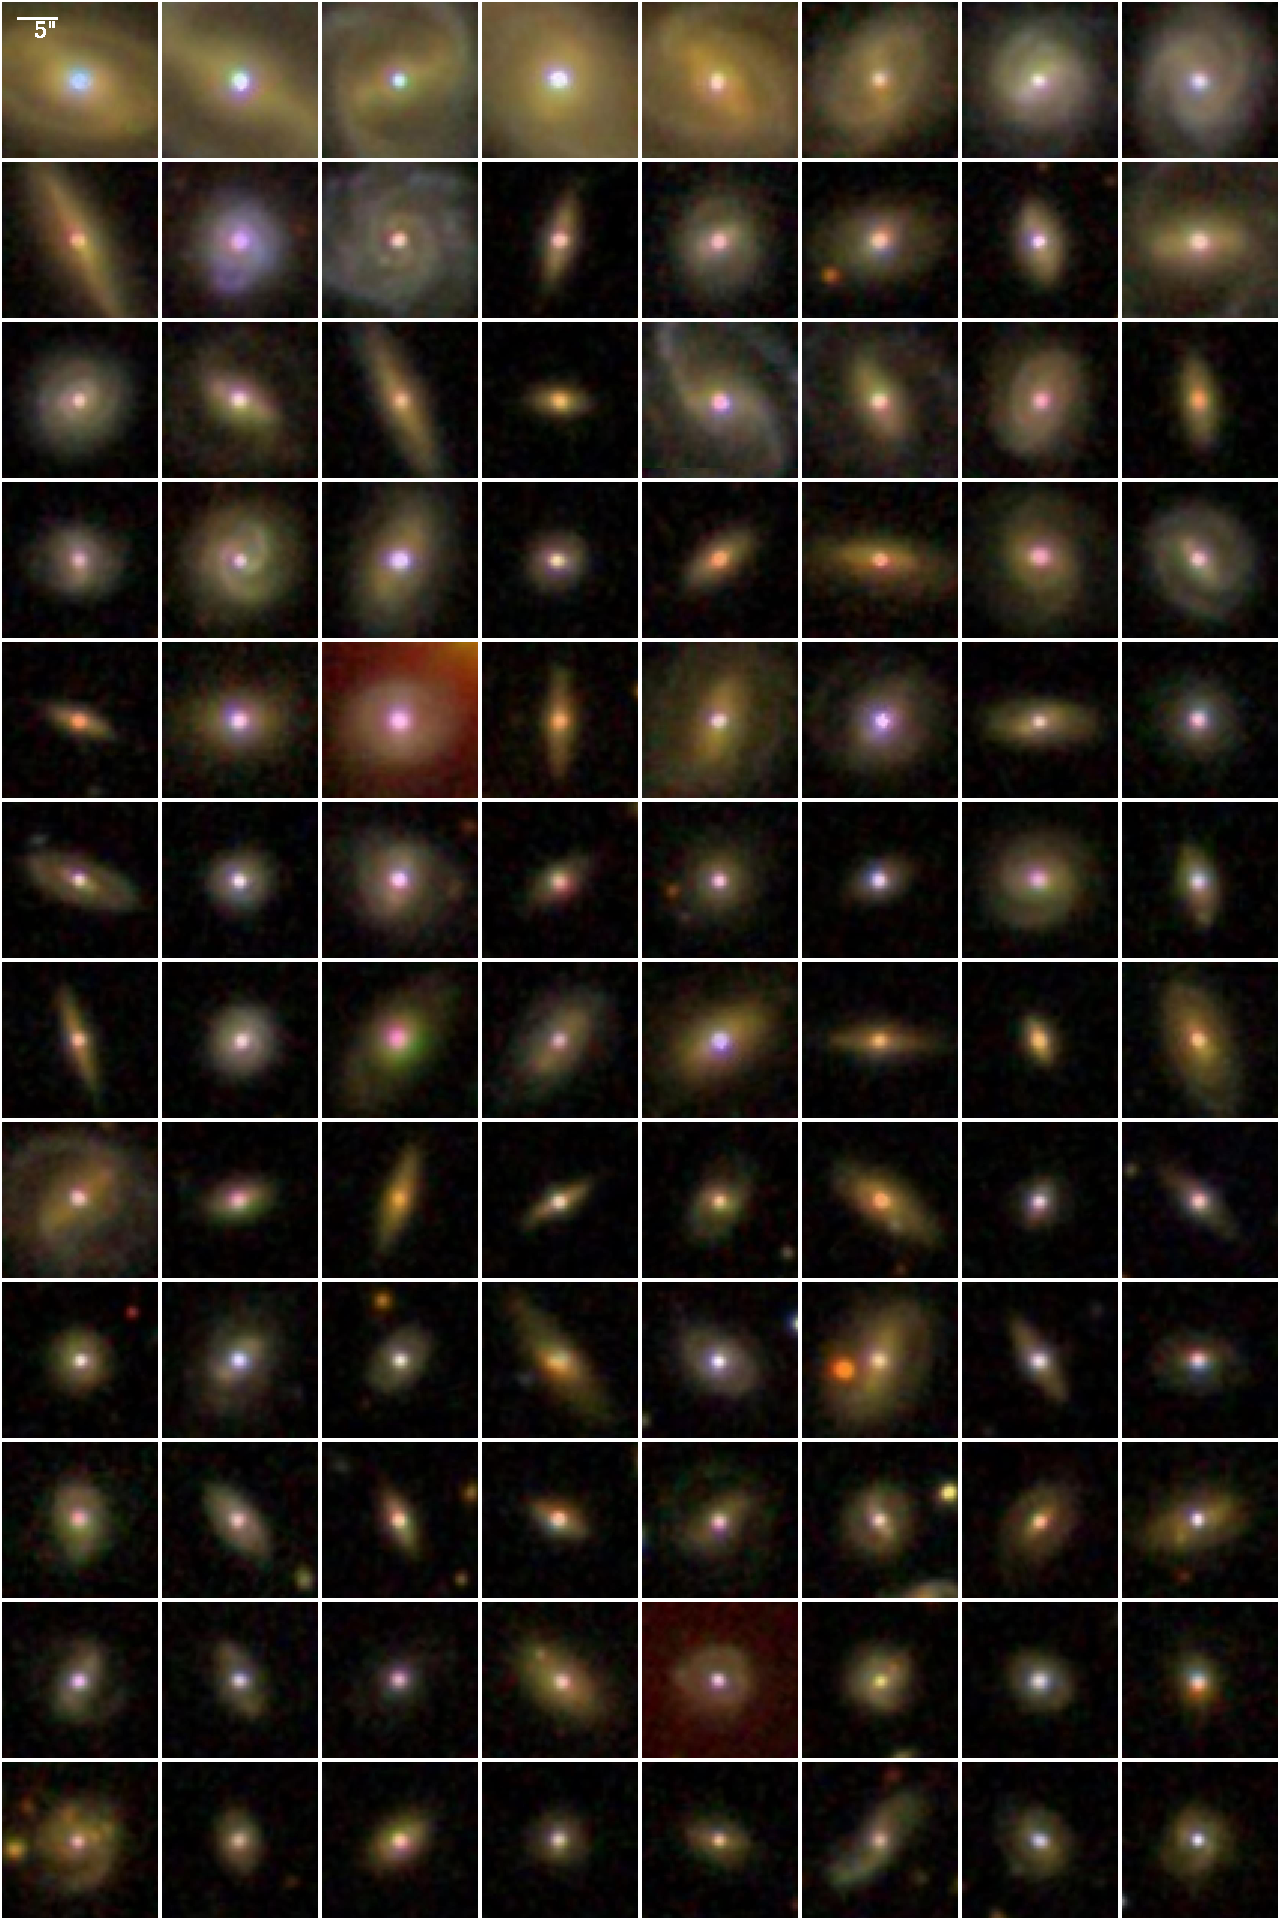
\includegraphics[height=0.9\textheight]{agn/mosaic_all_diskdom_zsort.pdf}
\caption[SDSS images of DISKDOM sample]{Postage stamp SDSS images of the $96$ galaxies within the \textsc{discdom} sample for which SDSS spectra were available, sorted from lowest redshift ($z=0.03$; top left) to highest redshift ($z=0.24$; bottom right). The scale for each image is shown by the $5$'' ruler in the top left panel.}
\label{fig:exampleimages}
\end{figure*}


\begin{figure*}
\centering
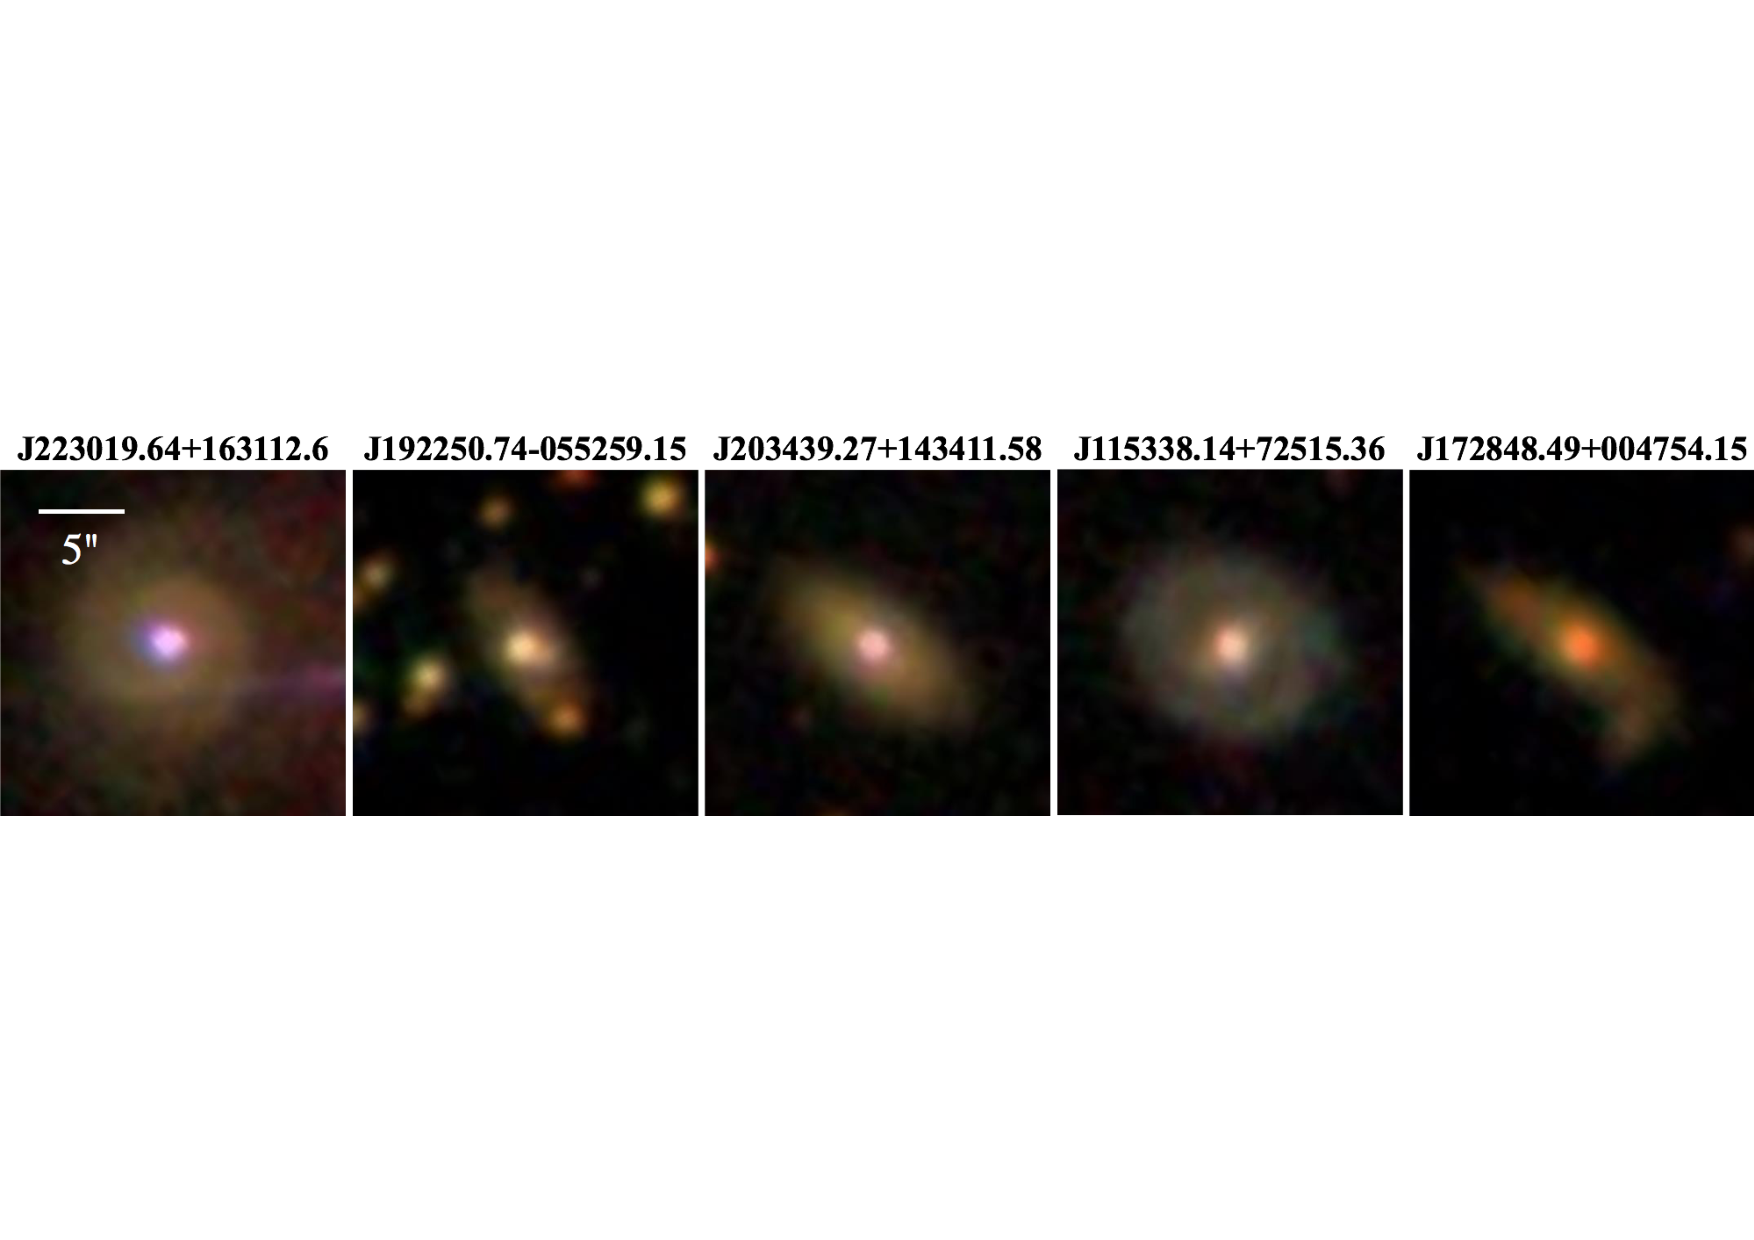
\includegraphics[width=\textwidth]{agn/mosaic_INT_gal_only.pdf}
\caption[SDSS images of 5 galaxies observed with the IDS on the INT]{Postage stamp SDSS images of the $5$ galaxies observed with the IDS on the INT within the \textsc{discdom} sample. The scale for each image is shown by the $5$'' ruler in the left panel.}
\label{fig:INTimages}
\end{figure*}


Following this selection of $4,316$ sources, galaxies imaged by the Sloan Digital Sky Survey are then further sub-selected. There are $1,844$ W2R sources with positional matches having reported coordinates within $3^{\prime \prime}$ of a source in the SDSS \citep{york00} Data Release 8, a fraction consistent with the fractional area of the SDSS versus an all-sky catalog. %76 per cent of this sub-sample have measured redshifts, with a peak redshift distribution of $z \approx 0.12$.  90 percent of sources with redshifts have $z < 0.6$; the distribution has a long tail to $z_{\rm max} = 2.35$.

Each of the $1, 844$ SDSS ugriz colour images were then examined to identify disc-dominated features. 101 disc-dominated AGN host galaxies were identified on the basis of clearly identifiable spiral arms, bars or obvious edge-on discs. I shall refer to these galaxies as the \textsc{discdom} sample. Figures~\ref{fig:exampleimages} \& \ref{fig:INTimages} collectively show the SDSS postage stamps for all galaxies in the sample, with all images showing the expected bright nebular emission of the unobscured AGN. 

%%%%%%%%%%%%%%%%%%%%%%%%%%%%%%%%%%%%%%%%%%%%%%
\subsubsection{Spectra}\label{sec:spectra}
%%%%%%%%%%%%%%%%%%%%%%%%%%%%%%%%%%%%%%%%%%%%%%

Of the 101 disc-dominated AGN host galaxies with SDSS imaging, 96 have spectra from SDSS Data Release 9 \citep{ahn12}. 23 of which were first identified as AGN by \cite{shen08} and \cite{edelson12}. Example spectra centred around the broad $H\alpha$ emission at $6562\AA$ for 5 of these SDSS spectra are shown in Figure~\ref{fig:SDSSspectra}.

\begin{figure*}
\centering
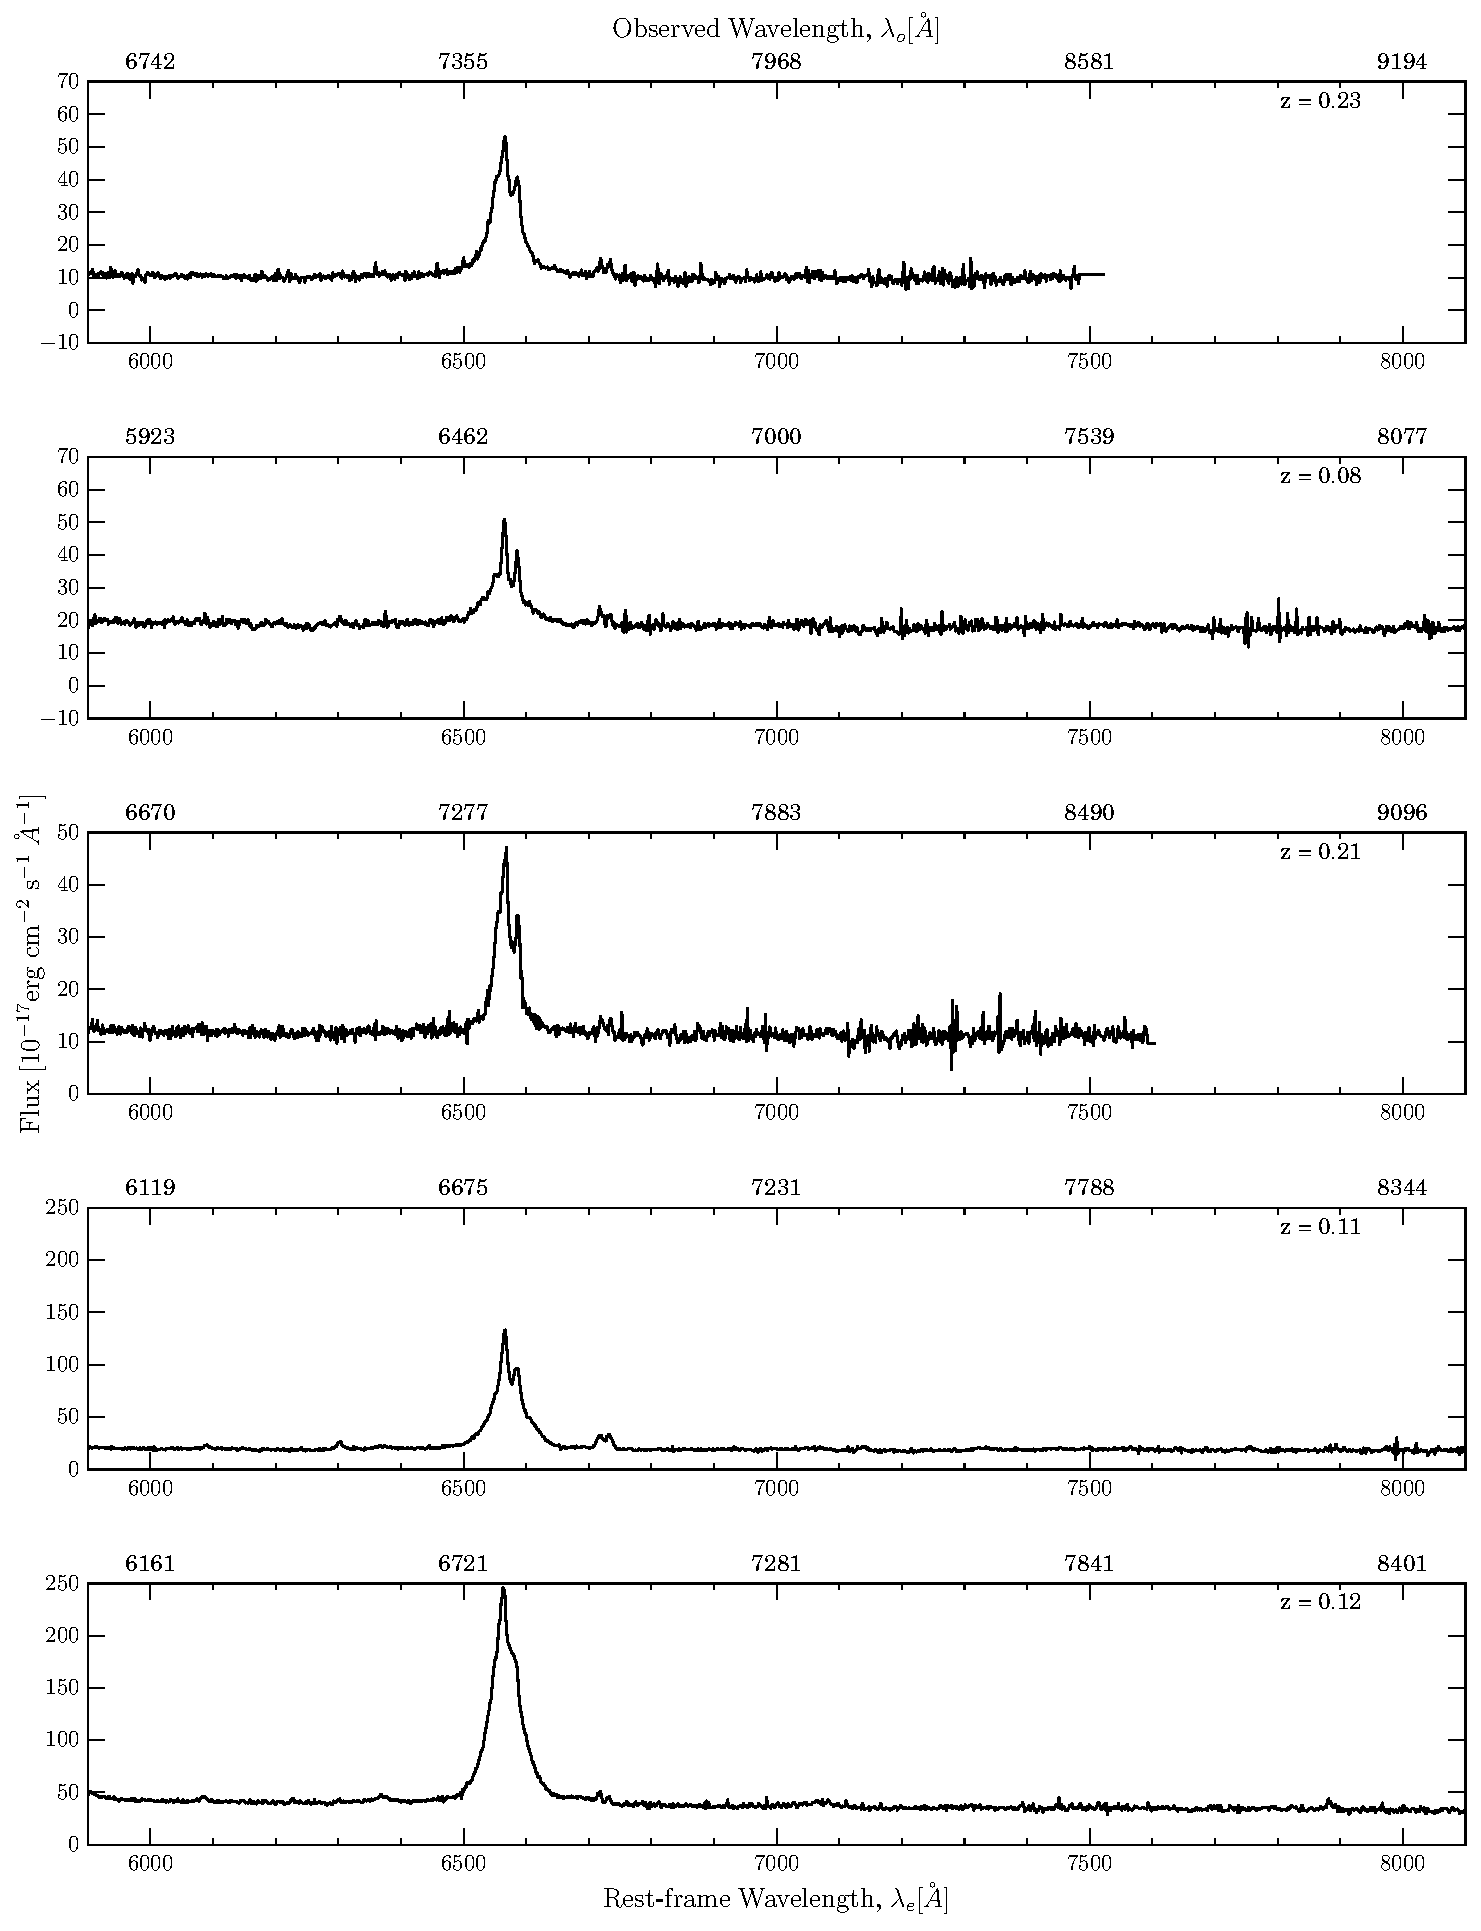
\includegraphics[height=0.8\textheight]{agn/sample_sdss_spectra.pdf}
\caption[Optical SDSS spectra of 5 galaxies in the DISKDOM sample]{5 example SDSS spectra from with the corresponding measured redshift values shown. Each panel shows the same rest-frame wavelength range (bottom axis of each panel); observed wavelengths are shown on the top axis of each panel. All spectra show broadened  $H\alpha$ emission, confirming that the multi-wavelength AGN selection employed here efficiently selects unobscured AGN.}
\label{fig:SDSSspectra}
\end{figure*}

The broad $H\alpha$ emission for  {\notebsm 5 additional sources} was measured using long-slit spectra techniques with the Intermediate Dispersion Spectrograph (IDS) on the Isaac Newton Telescope (INT) from 21st-23rd May 2014. I reduced these spectra using the standard reduction pipeline of Massey, Valdes \& Barnes (1992) using IRAF modules to debiase, dark subtract, flat field, calibrate, sky subtract, flux calibrate and finally extract spectra for the central regions of each galaxy. The redshift of these sources was also measured from the reduced spectra, using the peak of the broadened $H\alpha$ emission to measure $\lambda_{obs}$. These reduced spectra, centred around the broad $H\alpha$ emission at $6563\AA$, are shown in Figure \ref{fig:INTspectra} for the 5 galaxies observed.


\begin{figure*}
\centering
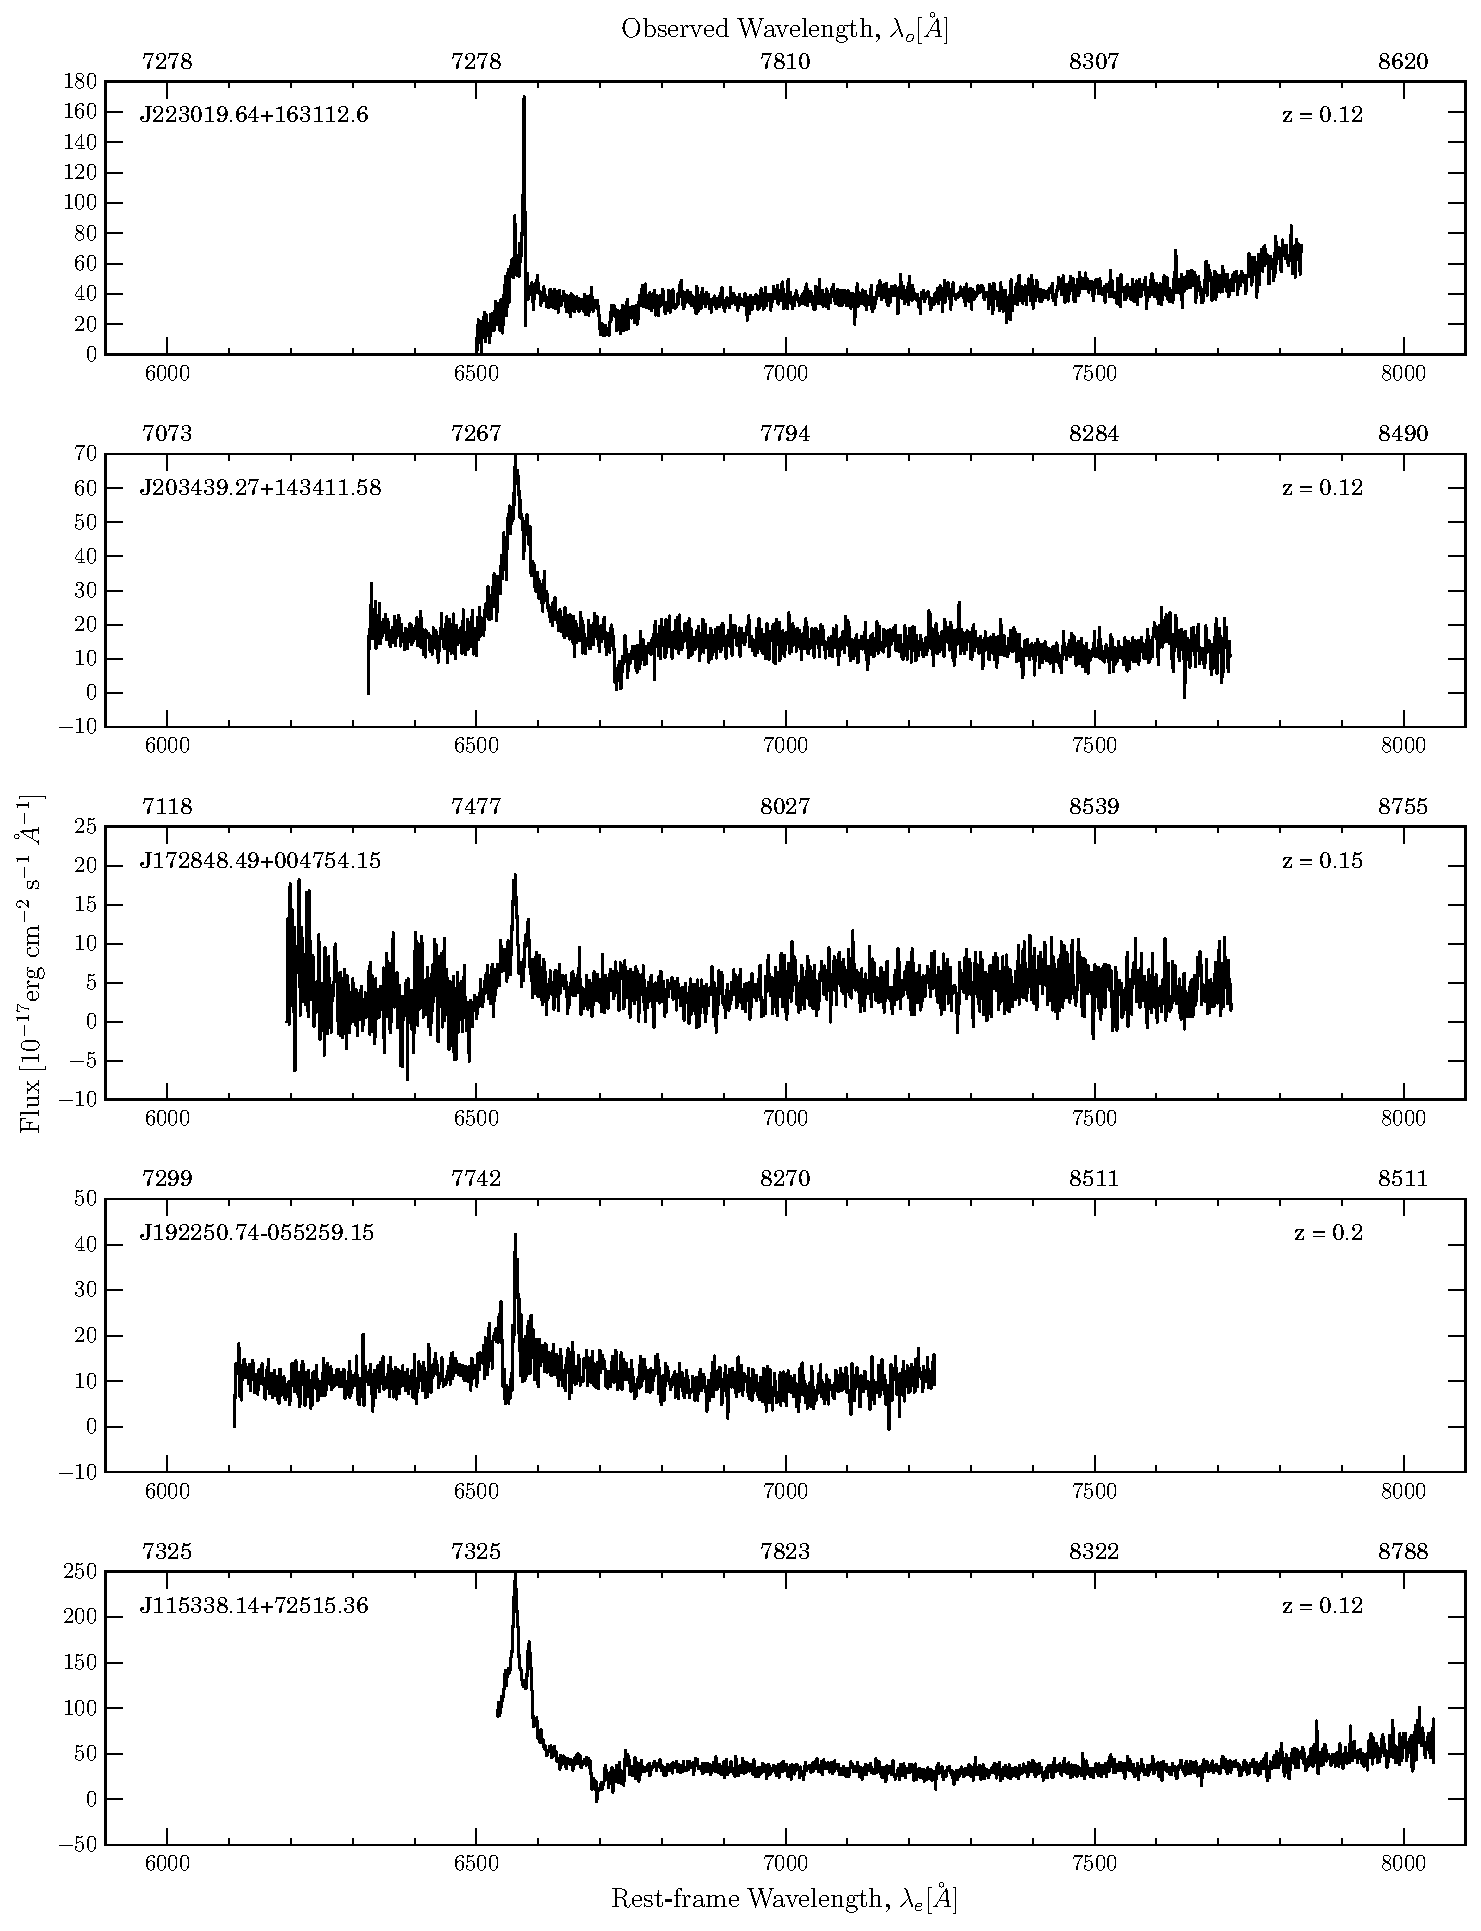
\includegraphics[height=0.8\textheight]{agn/int_spectra.pdf}
\caption[Optical spectra of 5 bulgeless galaxies observed on the INT with the IDS]{Reduced spectra from the IDS on the INT for the 5 galaxies observed. Each panel shows the same rest-frame wavelength range (bottom axis of each panel); observed wavelengths are shown on the top axis of each panel, with redshifts in the top right of each panel. All spectra one again show broadened $H\alpha$ emission, confirming that the multi-wavelength AGN selection employed here efficiently selects unobscured AGN.}
\label{fig:INTspectra}
\end{figure*}

% maybe some details about the spectral resolution?

Figure \ref{fig:redshifts} shows the redshift distribution of all 101 sources for which we have spectra; the mean redshift of the sample is $\left< z \right> = 0.129$, with the highest-redshift source having $z = 0.244$. 


\begin{figure}
\centering
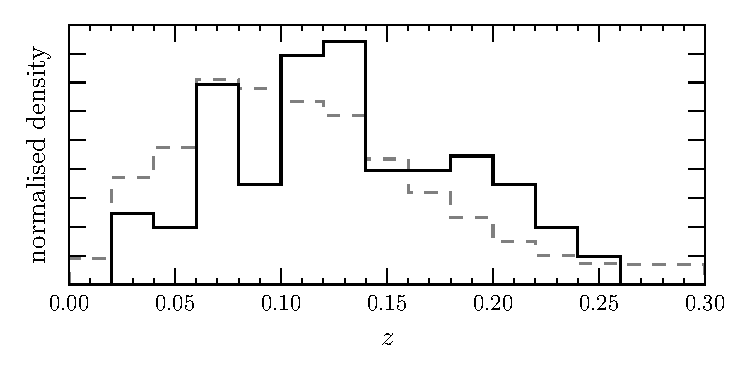
\includegraphics[width=0.9\textwidth]{agn/z_distribution_101_sdss.pdf}
\caption[Redshift distribution of bulgeless galaxies]{Normalised redshift distribution for all 101 sources (solid) for which we have spectra, either from SDSS or measurements with the IDS on the INT. Also shown is the overall redshift distribution of SDSS DR7 in the relevant redshift range of our sources (dashed).
}
\label{fig:redshifts}
\end{figure}

\subsubsection{Selecting a Control Sample}

Since the majority of the galaxies in the \textsc{discdom} sample have been observed using SDSS, I constructed a control sample from the SDSS quasar catalog of \citet{shen11}. Using this sample I compiled a sample of 191 galaxies which were redshift matched to within $\pm5\%$ of the \textsc{discdom} sample. I shall refer to these galaxies as the \textsc{qsocontrol} sample. 124 of the \textsc{qsocontrol} sample also had measured $(B/T)_r$ ratios from \citet[][matched with a $3''$ search radius, see Section~\ref{sec:galmass}]{simard11}. 

This provides a control sample of `typical' AGN host galaxies representative of the population in the redshift range probed in this study. 

%%%%%%%%%%%%%%%%%%%%%%%%%%%%%%%%%%%%%%%%%%%%%%
%
%
\subsection{Galaxy and Black Hole Properties}\label{sec:masses}
%
%
%%%%%%%%%%%%%%%%%%%%%%%%%%%%%%%%%%%%%%%%%%%%%%

In order to study the relation between the galaxies and their SMBHs in these disc dominated systems, their properties shall be compared to well tested black hole-galaxy scaling relations. In the following section I therefore describe how the photometry, black hole masses, total and bulge stellar masses, bolometric luminosities and Eddington ratios were derived for each galaxy in the \textsc{discdom} sample. 

\subsubsection{Photometry}\label{sec:photo}

The AGN contribution to the magnitude of each galaxy, $m_{\rm{gal}}$, is calculated by subtracting the flux in the SDSS {\tt psfMag}, $m_{\rm{psf}}$, from the flux in {\notebsm {\tt modelMag}}, $m_{\rm{model}}$ in a given wave band, $b$ as follows:

\begin{equation}\label{galmag}
m_{\rm{b, gal}} = -2.5 \log_{10} \left[ 10^{\left(\frac{m_{\rm{b, model}}}{-2.5}\right)} - 10^{\left(\frac{m_{\rm{b, psf}}}{-2.5}\right)} \right],
\end{equation}

since the normalisation constants in the flux-magnitude conversion will be constant for different sized apertures in a given band. {\tt psfMag} is the best estimate of unresolved emission, while {\tt modelMag} is the optimal quantity for computing aperture-matched source colours\footnote{https://www.sdss3.org/dr10/algorithms/magnitudes.php}. A galaxy magnitude in both the SDSS $u$ and $r$ bands was calculated in order to determine the galaxy $u-r$ colour. 

A similar NUV galaxy magnitude can be calculated using the GALEX apertures, however matching these apertures to those provided by SDSS cannot be done with a large enough degree of accuracy to derive a reliable galaxy $NUV-u$ colour. This therefore means that \textsc{starpy} cannot be run on these unobscured AGN host galaxies of the \textsc{discdom} sample. However, the locations of the \textsc{discdom} sample on the optical colour-magnitude diagram can still be explored; this is studied in Section~\ref{sec:results} (see Figure~\ref{fig:cmdmdot}). 

%%%%%%%%%%%%%%%%%%%%%%%%%%%%%%%%%%%%%%%%%%%%%%
\subsubsection{Total stellar masses}\label{sec:galmass}
%%%%%%%%%%%%%%%%%%%%%%%%%%%%%%%%%%%%%%%%%%%%%%

Total stellar masses are calculated using the well-studied relation between stellar mass, absolute galaxy $r$-band magnitude, $M_{\rm{r, gal}}$, and $u-r$ galaxy colour \citep[corrected for galactic extinction;][]{schlegel98}, following the method of \citet[][see Section \ref{intro}]{Baldry06}. Uncertainties are propagated from the colour-magnitude relationship and due to the subtraction of the central AGN component. The average uncertainty on each measurement is $\sim0.3~\rm{dex}$. The distribution of the stellar masses calculated for the \textsc{discdom} sample is shown in the right panel of Figure~\ref{fig:discdomdist}. 
% not sure if this modelMag vs petroMag vs cModelMag will also be in e.g. Strauss et al. (2002)... must find someone to ask

\subsubsection{Bulge stellar masses}\label{sec:bulgemass}

Calculation of the bulge stellar mass for the \textsc{discdom} sample is more complicated than the total stellar mass calculation described in the previous section. The nuclear emission (as estimated via comparison of {\tt psfMag} to {\tt modelMag}) is generally between {\notebsm 20 to 200 per cent} of the galaxy-only emission. The presence of the luminous AGN therefore severely compromises the estimates of the bulge-to-total ratio, $(B/T)$, in the host galaxy provided by, e.g., the {\tt fracDeV} parameter reported in the SDSS catalogs. The {\tt fracDeV} parameter estimates that $\sim 80\%$ of the galaxies in this sample are pure \citet{devaucouleurs} bulges in the $r$-band, despite the fact that the sample was selected on the basis of clear visual signatures of dominant discs (see Figure \ref{fig:exampleimages}). None of the photometric parameters derived by the SDSS pipeline allow for the dual presence of an AGN and a host galaxy. Without such considerations the unresolved AGN light is likely to be attributed to the compact bulge component in a bulge-disc model fit \citep{simmons08,koss11} leading to an overestimate of the bulge stellar mass.


\begin{figure*}
\centering
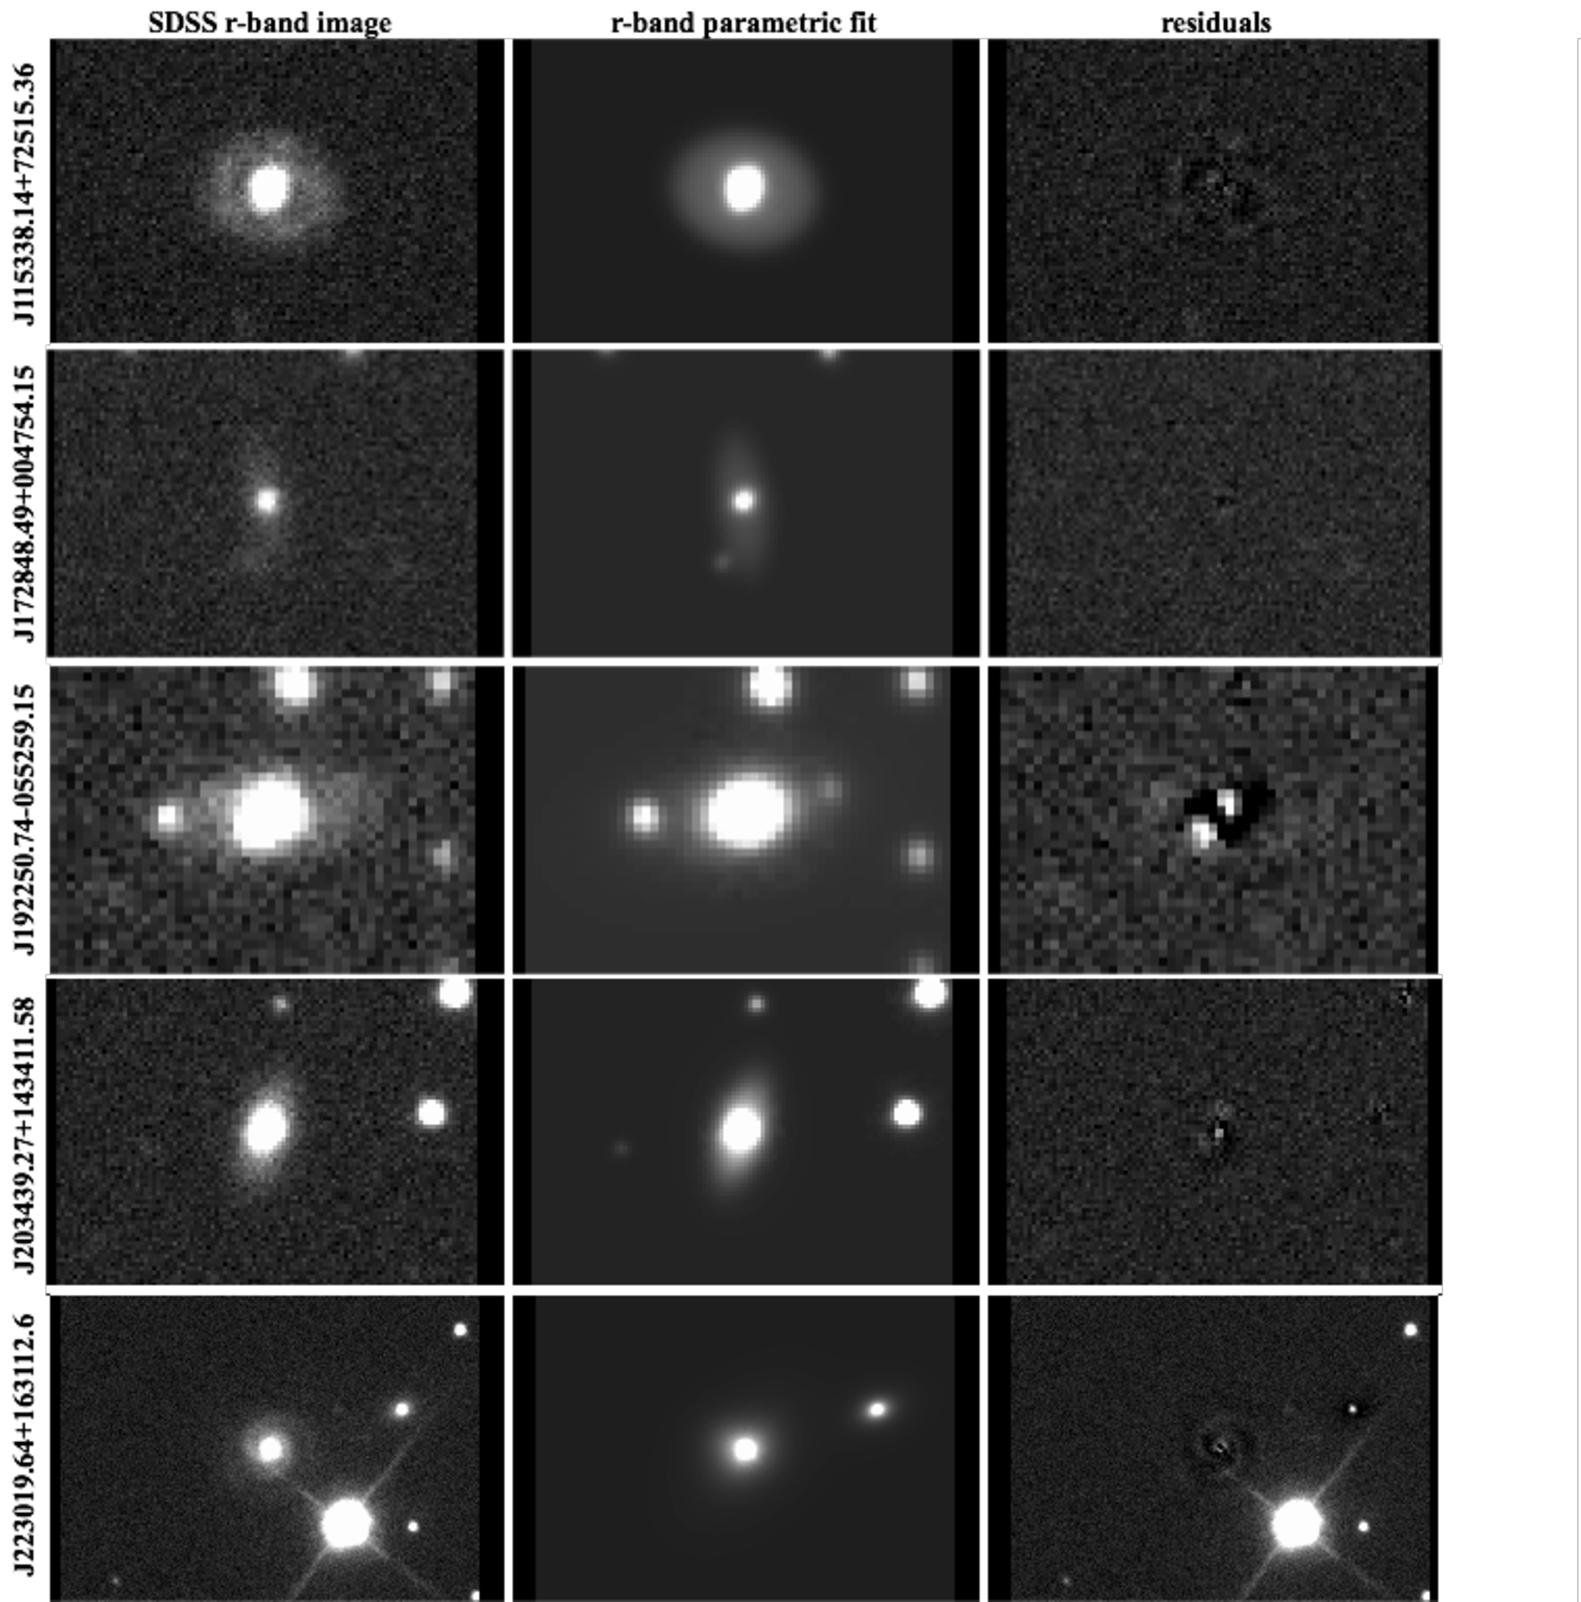
\includegraphics[width=\textwidth]{agn/galfit_residuals.pdf}
\caption[Parametric fits and residuals for the 5 galaxies observed at the INT]{SDSS r-band images (left), with the 3 component parametric fits from GALFIT (middle) and the residuals (right; with the same scale as the original image) for the 5 galaxies observed with the IDS on the INT. Stable, but uncertain, bulge-to-total ratios were only recovered for the galaxies in the top two rows. In the bottom three rows the nuclear emission was too bright and image resolution too low to derive a reliable estimate of the bulge-to-total ratio.
}
\label{fig:galfit}
\end{figure*}

% wherever the first mention of a pseudo-bulge is, need to \citep{kormendy04}.
AGN-host decomposition based on 2-dimensional image fitting \citep[e.g.,][]{simard98,peng02,peng10} is more reliable \citep[e.g.][]{mclure99,urry00,mclure01,sanchez04,pierce07,gabor09,Simmons11,Simmons13,koss11}. However even in high-resolution \emph{Hubble Space Telescope (HST)} images \citep{simmons08} or SDSS imaging at $z \gtrsim 0.06$ \citep[][]{koss11,Simmons13} the recovered bulge-to-total ratio can be highly uncertain, particularly for disc-dominated galaxies with a very small bulge or pseudo-bulge \citep{kormendy04} component. While the AGN-host decompositions of the galaxies studied by \citet{Simmons13} recovered reliable bulge-to-total ratios for 11 of the 13 galaxies, their sources were at substantially lower redshift than the \textsc{discdom} sample (with the majority at $z < 0.08$), and their AGN significantly less luminous ($L_{bol} \lesssim 10^{44} \rm{erg}~\rm{s}^{-1}$, whereas in the \textsc{discdom} sample $L_{bol} \gtrsim 10^{44} \rm{erg}~\rm{s}^{-1}$, see Section~\ref{sec:eddratios}). 

Bulge-to-total fits were first attempted for the 5 galaxies in the \textsc{discdom} sample which were observed with the IDS on the INT using the \textsc{galfit} software \citep{peng02}; the results of which are shown in Figure~\ref{fig:galfit}. I used a S\'ersic light profile \citep{sersic68} to model bulge and disc components, defined by an effective radius, $R_e$, and light concentration index, $n$, as:
\begin{equation}\label{sersic}
I(R) = I_e \exp \left(  -b_n \left[  \left( \frac{R}{R_e}\right)^{1/n} -1 \right] \right),
\end{equation}
where $I_e$ is the intensity at the effective radius, $R_e$ and $b_n$ is a constant defined in relation to the S\'ersic index, $n$. Typical disc (bulge) light profiles have $n\approxeq1$ ($n\approxeq3$). Each of the galaxies observed with the INT were fitted with a disc, bulge and PSF component (to account for the bright nuclear emission of the AGN). PSFs were extracted from the SDSS FITS images using the standard \texttt{read\_PSF} IDL code provided by the SDSS pipeline\footnote{\url{http://www.sdss.org/dr12/algorithms/read_psf/}}. Initial guesses of $n=2.5$ are used on the first pass of the \textsc{galfit} algorithm, which uses a $\chi^2$ minimisation method to determine the best fit S\'ersic index, effective radius, magnitude and position for each of the 3 components. This first pass allows the positions of the components to be determined, which are then fixed on a second pass of the algorithm to ensure accurate magnitudes, radii and S\'ersic indices are then inferred. From these models, the \textsc{galfit} r band magnitudes of the bulge, $m_{r, \rm{bulge}}$, and disc, $m_{r, \rm{disc}}$, components were used to calculate the bulge-to-total ratio, $(B/T)_r$, as follows:
\begin{equation}\label{btratio}
(B/T)_r = \frac{10^{(\frac{m_{r, \rm{bulge}}}{-2.5})}}{\left[10^{(\frac{m_{r, \rm{bulge}}}{-2.5})} + 10^{(\frac{m_{r, \rm{disc}}}{-2.5})}\right]}.
\end{equation}

Stable, but highly uncertain, bulge-to-total ratios were recovered for only {\notebsm 2} of the 5 galaxies (the top two rows in Figure~\ref{fig:galfit}). In the remaining 3 cases the nuclear emission was too bright and the image resolution too low for a reliable bulge-to-disc decomposition.  Detailed AGN host fits to the SDSS images in the rest of the \textsc{discdom} sample, which lie at similar redshifts, are therefore not likely to produce useful measurements of bulge masses. \emph{HST} imaging would enable these measurements, and although currently not available for the galaxies in this sample, observations are currently underway in Cycle 24 (ID: 14606). 

Nevertheless, it is possible to constrain the bulge contribution to the host galaxies using existing structural parameters from large-scale studies performing bulge-disc decompositions of SDSS galaxies. While such studies do not account for the presence of an AGN, their tendency to overestimate the bulge-to-total ratio as a result means that bulge masses derived from these quantities may be taken to be conservative upper limits.

\citet{simard11} fit multiple models to 1.12 million galaxies in the SDSS catalog to determine best-fit structural parameters for each galaxy. Their $r$-band bulge-to-total ratio {\notebsm of the best-fit model} is taken as an upper limit to the true bulge-to-total ratio of the \textsc{discdom} sample. To convert limits on bulge luminosities to limits on bulge masses, we assume the mass-to-light ratio of the bulge is equal to the mass-to-light ratio of the disc. This is a reasonable assumption for disc-dominated galaxies, where many of the ``bulge'' components, if present, are likely to be rotationally-supported pseudo-bulges \citep{kormendy04} with stellar populations similar to that of the disc {\notebsm \citep[e.g.,][]{graham01a}}.

The bulge-to-total ratio upper limits of the 89 galaxies in the \textsc{discdom} sample which were included in the \citet{simard11} study, range from {\notebsm $0.13 \leq \left({\rm B/Tot}\right)_{r, \rm max} \leq 1.0$, with a mean value of 0.5}. Inspection of the morphologies of the galaxies shown in the images in Figure~\ref{fig:exampleimages} reveals how such a range in $\left({\rm B/Tot}\right)_{r, \rm max}$ is clearly an overestimate of the bulge contribution to these galaxies. Applying these bulge-to-total limits to the stellar masses derived in Section~\ref{sec:galmass}, results in bulge mass upper limits of {\notebsm $3 \times 10^9 \mmsun < {\rm M_{bulge}} < 7 \times 10^{10} \mmsun $}. The distribution of bulge-to-total ratios in the \textsc{discdom} sample are shown in the middle panel of Figure \ref{fig:discdomdist}

%%%%%%%%%%%%%%%%%%%%%%%%%%%%%%%%%%%%%%%%%%%%%%
\subsubsection{Black hole mass estimates}\label{sec:bhmass}
%%%%%%%%%%%%%%%%%%%%%%%%%%%%%%%%%%%%%%%%%%%%%%

The selection of unobscured AGN facilitates the accurate estimate of black hole masses using a viral assumption. Unobscured AGN have broad emission lines originating from within the black hole sphere of influence; this photoionized broad line region (BLR) can be used as a dynamical tracer of the black hole mass. The viral black hole mass \citep{peterson14} can be expressed simply as:
\begin{equation}\label{eq:virial}
M_{BH} = f \frac{R\Delta v^2}{G},
\end{equation}
where $\Delta v$ is the velocity dispersion of the emitting BLR, which is assumed to be spherical with radius $R$. The factor, $f = 0.75$ \citep{netzer90} then corrects for this simplifying assumption. The velocity dispersion of the BLR can be inferred from the FWHM of a broad line, such as $H\alpha$ or $H\beta$, and the radius inferred from the luminosity of the same broad line. This radius-luminosity relationship is calibrated using the more precise black hole mass measurement technique of reverberation mapping \citep{blandford82, peterson01, barth15} in which the radii are measured based on the observed delay between variations in the AGN continuum and the BLR emission \citep{kaspi05, bentz06}. Masses derived with this virial method, under these simplifying geometric assumptions, have been shown to be accrate to within a factor of $\sim 3$ when compared to masses derived using the $M_{BH}$-$\sigma$ method \citep[][and see Section~\ref{agnsample}]{ferrarese01, nelson04, onken04}.

Using the $M_{BH}$-$\sigma$ relation to calculate black hole masses (as in Section~\ref{agnsample}) is not possible in this case since I am trying to investigate how these galaxies evolve in comparison to the `typical' AGN host galaxy population used to fit the $M_{BH}$-$\sigma$ relation. Instead I employ the established relation between the black hole mass and the FWHM and luminosity in the broad \ha\ line of \citet{gh07a}: 
\begin{equation}\label{greeneho}
M_{BH} = (3.0^{+0.6}_{-0.5}) \times 10^6 \left ( \frac{L_{H\alpha}}{10^{42} ~\rm{erg}~\rm{s}^{-1}} \right )^{0.45\pm0.03} \left ( \frac{\rm{FWHM}_{H\alpha}}{10^{3}~\rm{km}~\rm{s}^{-1}} \right )^{2.06\pm0.06} M_{\odot},
\end{equation}
derived using the virial method described above. 

To obtain an estimate of the FWHM of the broadened $H\alpha$ lines, I performed spectral fitting on each of the SDSS and INT spectra described in Section \ref{sec:spectra} to recover narrow- and broad-line strengths and widths of the $\mha\ 6563$ \AA\ line, by using \gandalf\ \citep{sarzi06} {\notebsm to fit multiple simultaneous lines as well as the continuum of the spectra}. \gandalf\ is optimised for use with SDSS spectra and so using the program with the INT spectra required minimal data re-formatting; I logarithmically re-binned and de-redshifted the spectra. {\notebsm From the continuum-subtracted best fit provided by \gandalf\}, I determine the FWHM and line flux of the broad and narrow components of the \ha\ line simultaneously, one again employing \emcee\footnote{\url{dan.iel.fm/emcee/}}, the Python MCMC ensemble sampler by \cite{emcee13}, described in Chapter~\ref{starpy}. 

The uncertainties reported by \emcee\ encapsulate the separation of narrow and broad line components in measurement of the FWHM. The reported uncertainties on black hole masses include this source of uncertainty as well as the reported uncertainties in the black hole-broad line relation \citep{gh07a}. There are other sources of uncertainties, such as those involved in implicitly assuming the fixed geometric correction factor, $f=0.75$ \citep{netzer90} for each SMBH, the spectral noise, and the error introduced by assuming a Gaussian line profile for all measured broad lines. Determining uncertainties for the last two is outside the scope of this study; based on visual inspection of the line fits, the first is very small compared to the other uncertainties. These fits to the broad and narrow line \ha \ components in the INT spectra are shown in Figure \ref{fig:zoomspectra}.

\begin{figure}
\centering
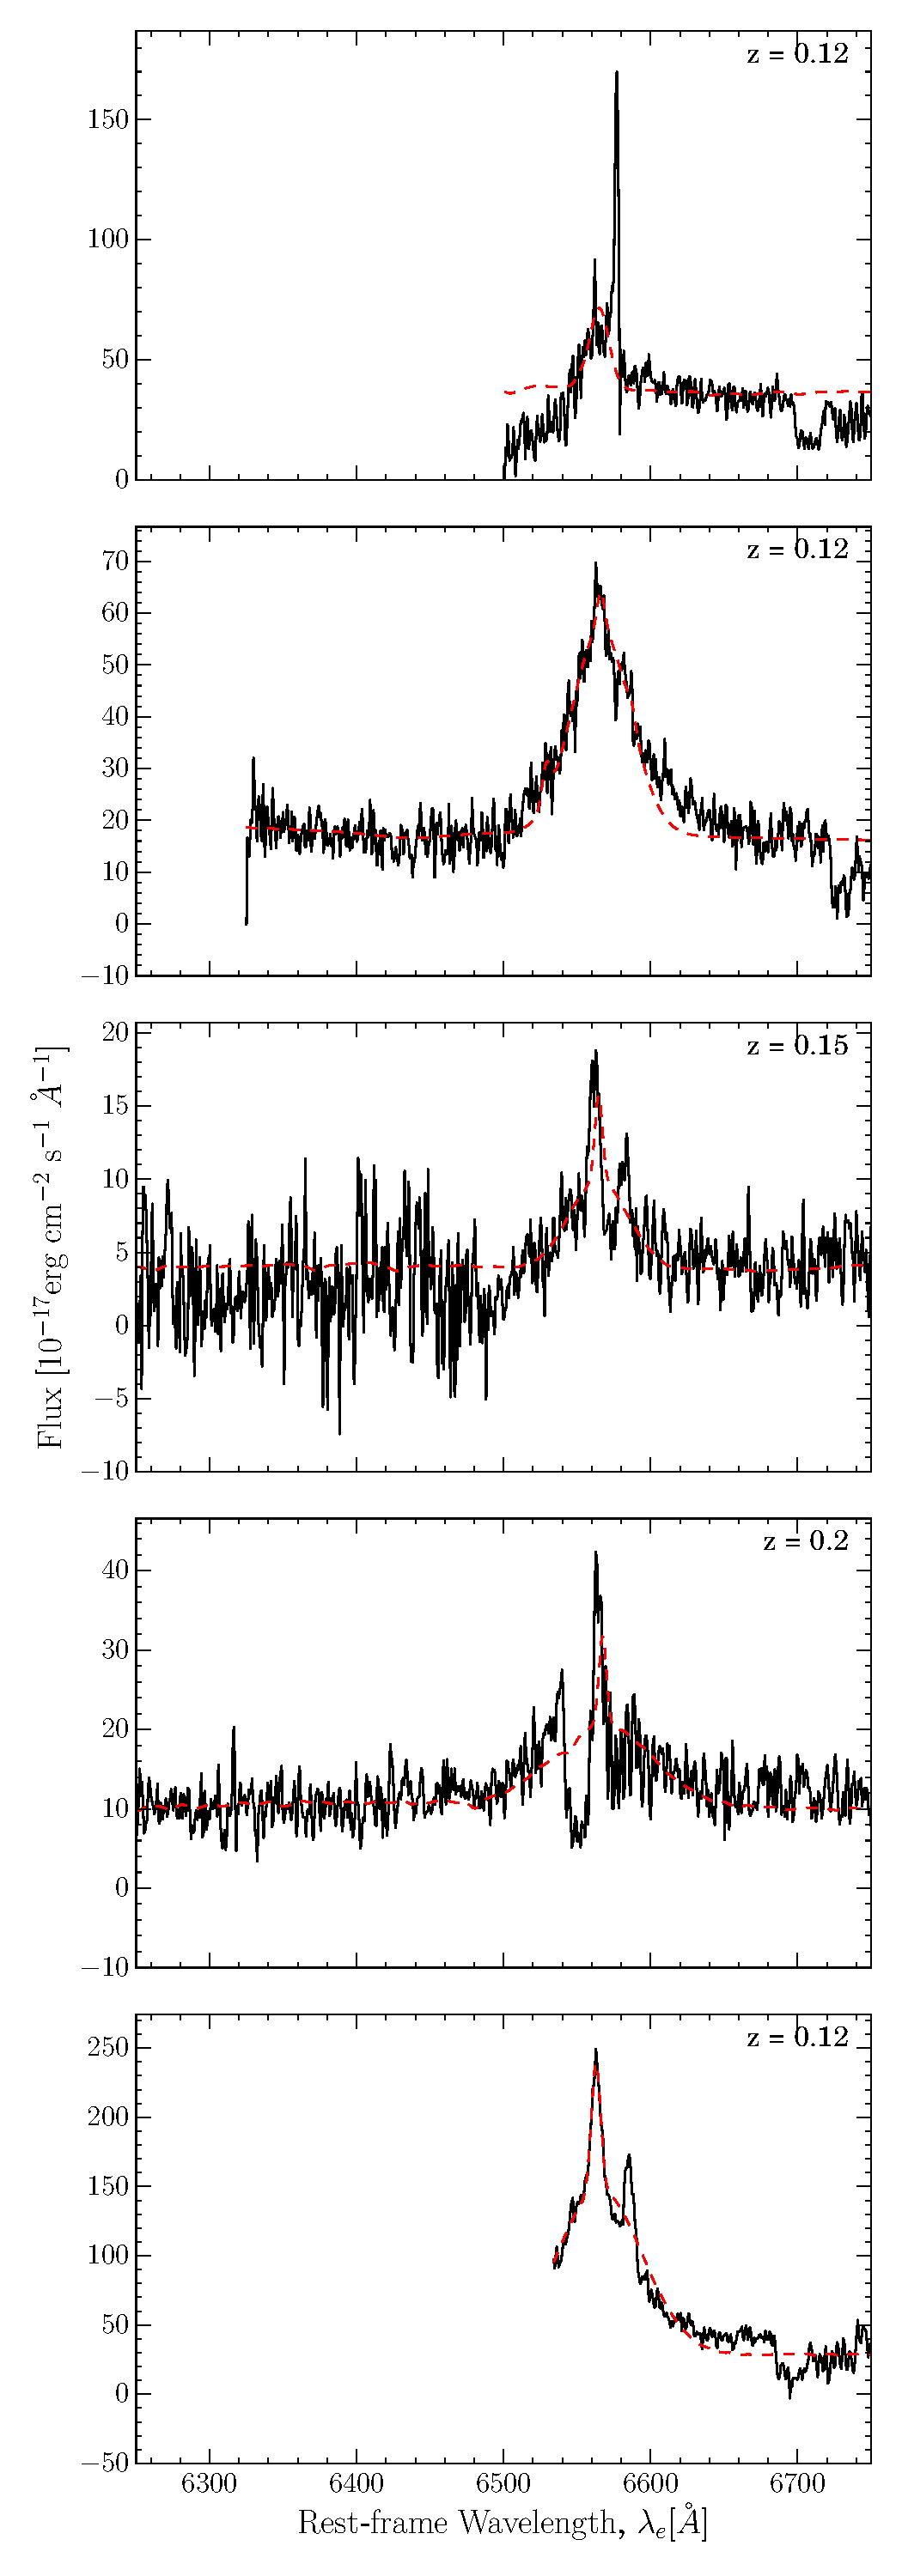
\includegraphics[height=0.9 \textheight]{agn/int_zoom_spectra.pdf}
\caption[Zoom in on $H\alpha$ region of the spectra of 5 galaxies observed with the IDS on the INT]{Reduced spectra from the IDS on the INT for the 5 galaxies observed with the corresponding measured redshift values shown. Spectra are aligned with the broad $H\alpha$ emission line, the gaussian fits to which are shown by the dashed red line.  }
\label{fig:zoomspectra}
\end{figure}

The black hole masses for the 101 galaxies of the \textsc{discdom} sample range from {\notebsm $10^6.2 \mmsun \leq \mmbh \leq 2 \times 10^9.5 \mmsun$} and the distribution is shown in the left panel of Figure~\ref{fig:discdomdist} in comparison to those from the \textsc{qsocontrol} sample. 

\subsubsection{Bolometric Luminosities}\label{sec:eddratios}

Bolometric luminosities are calculated from the wavelength-dependent bolometric corrections of \citet{richards06} using the conversion from the $12\mu m$ infrared luminosities, $ L_{12\mu m}$:
\begin{equation}
L_{bol} \approx 8 \times L_{12\mu m}.
\end{equation}
The infrared luminosity,  $L_{12\mu m}$, is calculated from the WISE W3 magnitudes, $M_{W3}$, for which all of the \textsc{discdom} sources have a detection, as follows:
\begin{equation}
L_{12\mu m} = \left(\frac{4\pi d^2}{10^{-2}~\rm{m}^2}\right)\left( \frac{c}{\lambda}\right) \left(\frac{F_{\nu, 0}}{1\times10^{23}~ \rm{Jy}} \right)10^{\left(\frac{M_{W3}}{-2.5}\right)}.
\end{equation}

The derived bolometric luminosities were first used to calculate Eddington ratios, $\lambda_{Edd}$, for the \textsc{discdom} sample (using the method outlined in Section~\ref{agnsample}), and then the black hole mass accretion rate, $\dot{m}$, using a simple matter to energy conversion:
\begin{equation}\label{eq:ltomdot}
L = \frac{E}{t} = f\cdot \frac{mc^2}{t},
\end{equation}
where $f =0.15$ \citep{elvis02}, is a lower limit on the radiative efficiency factor (i.e. what fraction of the accreted mass can be turned into radiated energy). The black hole mass accretion rate, $\dot{m}$ is therefore calculated as:
\begin{equation}\label{eq:mdot}
\frac{m}{t} = \left(\frac{\dot{m}}{\rm{M}_{\odot}~\rm{yr}^{-1}}\right) = \left( \frac{1.58\times 10^{-26}}{f} \right) \left( \frac{\rm{cm}~\rm{s}^{-1}}{c} \right)^2 \left( \frac{L_{\rm{bol}}}{\rm{erg}~\rm{s}^{-1}} \right).
\end{equation}

All of these derived galaxy and black hole properties of the \textsc{discdom} sample are now compared to those of \textsc{qsocontrol} sample in Section \ref{sec:results}.


\begin{figure*}
\centering
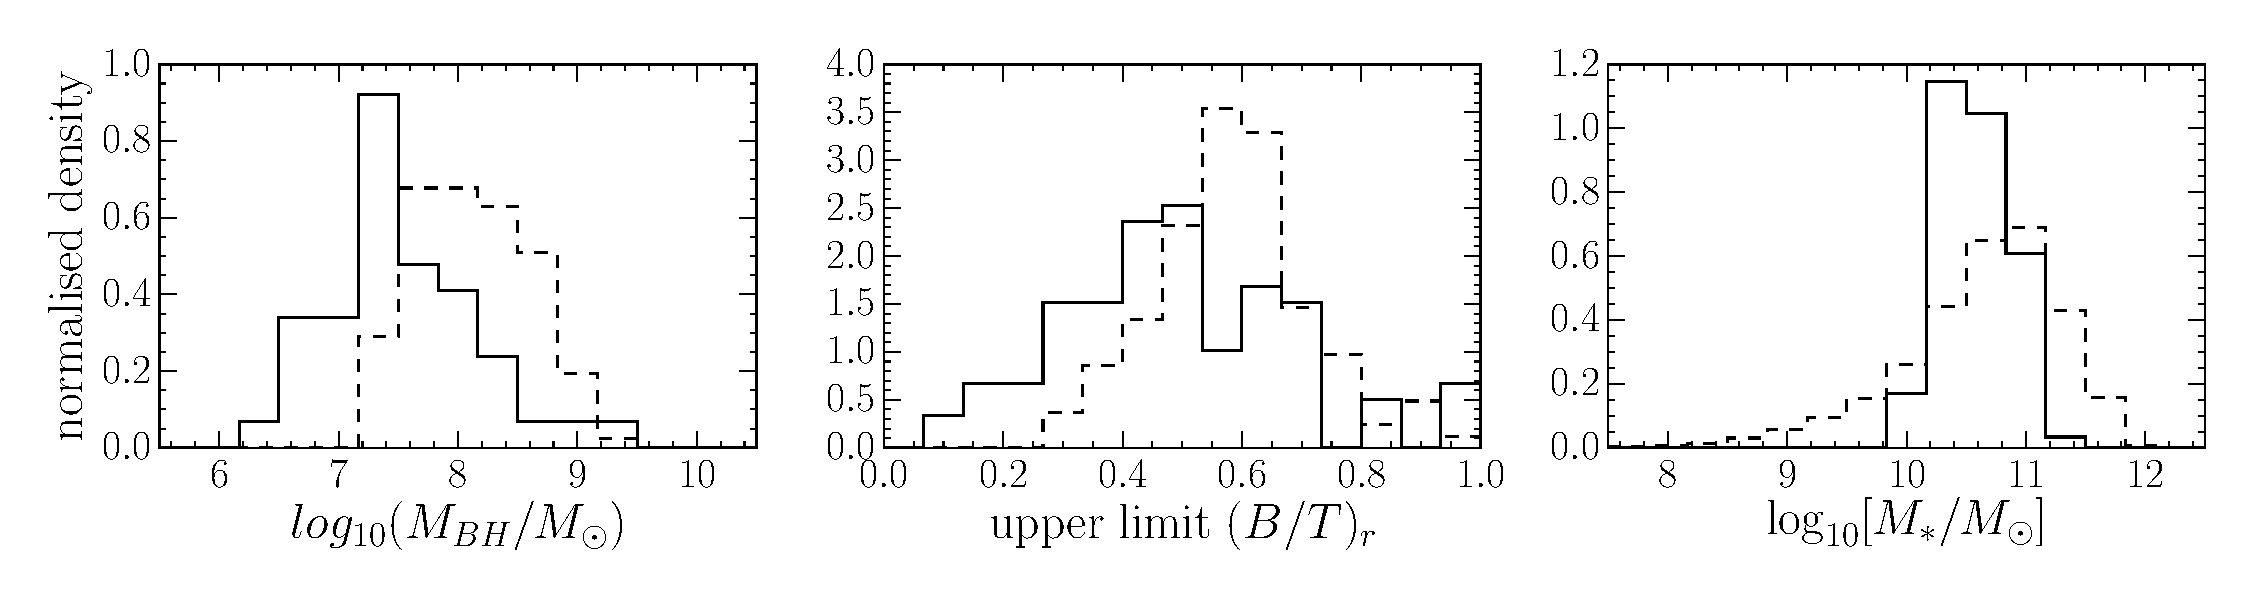
\includegraphics[width=\textwidth]{agn/diskdom_mbh_btot_stellar_mass_distributions.pdf}
\caption[Galaxy and black hole properties of the \textsc{discdom} sample in comparison to the \textsc{qsocontrol} sample]{Distributions of black hole mass (left), upper limits on the r-band bulge-to-total mass ratio from \citet[][middle]{simard11} and stellar mass (right) of the \textsc{discdom} sample (solid) in comparison to the \textsc{qsocontrol} sample (dashed).}
\label{fig:discdomdist}
\end{figure*}



%%%%%%%%%%%%%%%%%%%%%%%%%%%%%%%%%%%%%%%%%%%%%%
%
%  
\subsection{Results}\label{sec:results}
%
% 
%%%%%%%%%%%%%%%%%%%%%%%%%%%%%%%%%%%%%%%%%%%%%%



The total stellar mass and estimated bulge masses (see Section \ref{sec:galmass}) are plotted against the black hole masses for the \textsc{discdom} sample in Figures~\ref{fig:totvsbh} \& \ref{fig:bulgevsbh} respectively. I fit a multiple linear regression model to both of these relations using an inference method which encompasses the uncertainties on both $x$- and $y$-dimensions and the intrinsic scatter in the data. The full method is outlined in \citet{kelly07} and is publicly available as a \emph{Python} module \textsc{linmix}\footnote{\url{http://linmix.readthedocs.org/}}; a brief outline of the method is provided below. 

A multiple linear regression model assumes a simple linear relationship between two independent variables, $x$ and $y$, where both variables are unknown, with added noise, $\epsilon$, from an unknown unobserved random variable. In the \textsc{limmix} package this is modelled with the following form:
\begin{equation}\label{2dlinemodel}
\eta = \alpha + \beta * x_i + \epsilon
\end{equation}
\begin{equation}\label{2dlinemodel2}
x = x_i + x_{err}
\end{equation}
\begin{equation}\label{2dlinemodel3}
y = \eta + y_{err}.
\end{equation}
Here $\alpha$ and $\beta$ are the regression coefficients to be inferred (like $m$ and $c$ in a traditional $y=mx + c$ linear regression), $x_{err}$ is the error on the measured values $x_i$, and $y_{err}$ is the error on the measured values $\eta$. $\epsilon$ is assumed to be normally-distributed, centred around zero, with a variance $\sigma^2$. $x_{err}$ and $y_{err}$ are also assumed to be normally-distributed and centred around zero with variances $\sigma_x^2$ and $\sigma_y^2$, respectively and covariance $xy_{cov}$. This linear regression method can also incorporate the upper limits on the bulge mass measurements of the 89 SDSS galaxies measured by \citet[][see Section \ref{sec:galmass}]{simard11},  by treating them as `censored values' \citep[see Section 7.2 of][]{kelly07}, shown by the solid line in Figure~\ref{fig:bulgevsbh}.

Using \textsc{linmix}, I also fit to the observations of 30 early-type galaxies from \citet{haringrix04}. Despite the fact that galaxies in the \textsc{discdom} sample are disc dominated and contain either no bugle or a pseudo-bulge, they preferentially lie above the relationship between black hole and bulge stellar mass derived using the bulge dominated galaxies of \citet{haringrix04}, as seen in Figure~\ref{fig:bulgevsbh}. 

\begin{figure*}
\centering
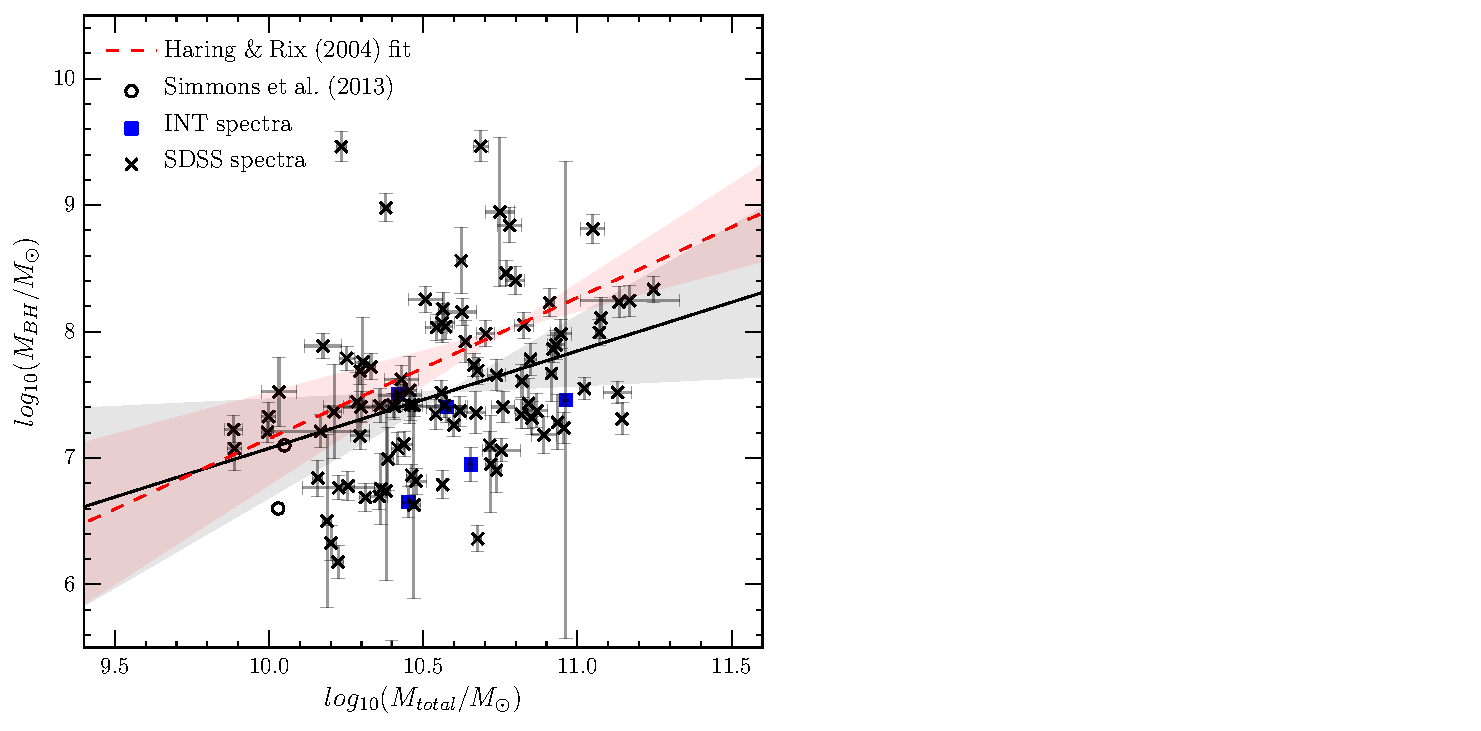
\includegraphics[width=\textwidth]{agn/mass_bh_total_mass_fit_linmix_fit.pdf}
\caption[Black hole stellar mass relation for the \textsc{discdom} sample]{Total stellar mass against the black hole mass of the 101 galaxies, including those observed by SDSS (crosses), with the IDS on INT (blue squares) and detections from \citet[open cirlces]{Simmons13}. The best fit line to the data points and two-dimensional errors from linear regression is shown (solid line) with $\pm3\sigma$ (grey shaded). I also show the best fit found using this same method to the early-type galaxies of \citet{haringrix04} (dashed line) with $\pm3\sigma$ (red shaded) and the measured values shown by the red circles. Despite the fact that these galaxies are predominantly disc dominated they are found in the same region of parameter space as the bulge dominated systems used to derive the \citet{haringrix04} relationship (see discussion in Section \ref{sec:intdiscussion}).
}
\label{fig:totvsbh}
\end{figure*}

\begin{figure*}
\centering
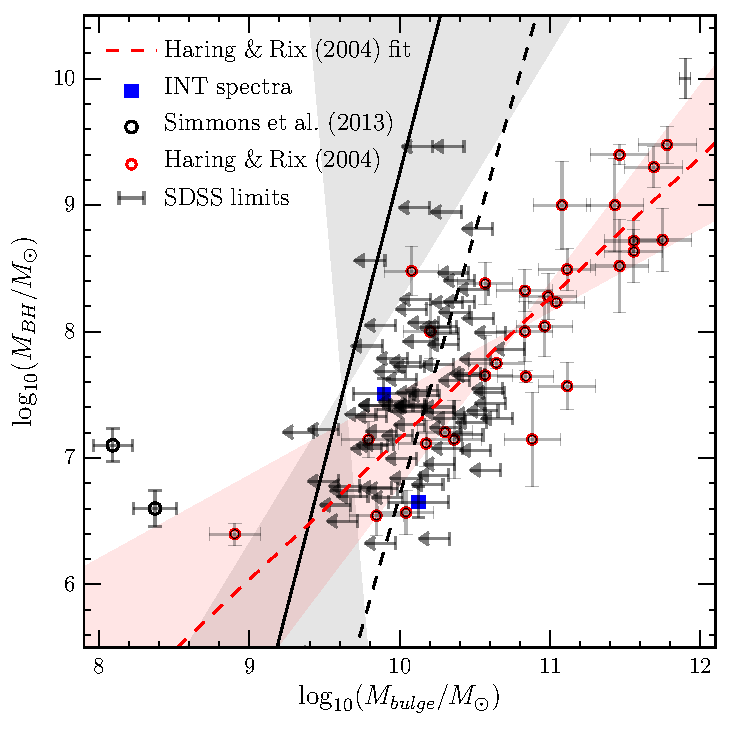
\includegraphics[width=\textwidth]{agn/mass_bh_bulge_limits_INT_simmons13_measurements_linmix_fit.pdf}
\caption[Black hole bulge mass relation for the \textsc{discdom} sample]{The upper limits on the calculated bulge masses are plotted against the black hole mass with the best fit to these upper limits and two-dimensional errors using linear regression methods (solid line) shown with $\pm3\sigma$ (grey shaded). The dashed line shows the fit if the upper limits are not treated as such. I also show the best fit found using this same method to the early-type galaxies of \citet{haringrix04} (dashed line) with $\pm3\sigma$ (red shaded) and the measured values shown by the red circles. Despite the fact that these galaxies are predominantly disc dominated they will are most likely to lie above the \citet{haringrix04} relationship found for bulge dominated systems (see discussion in Section \ref{sec:intdiscussion}).
}
\label{fig:bulgevsbh}
\end{figure*}

\begin{figure}
\centering
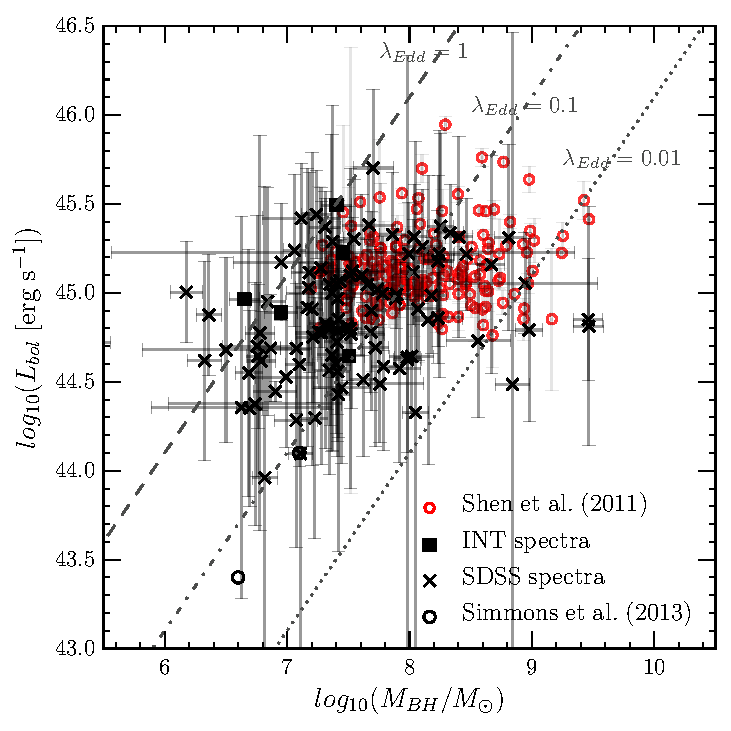
\includegraphics[width=\textwidth]{agn/mass_bh_bol_luminosity_with_all_errors_shen_11.pdf}
\caption[Black hole mass against luminosity for the bulgeless AGN sample]{Black hole mass against bolometric luminosity for the 101 galaxies, including those observed by SDSS (crosses) and with the IDS on INT (squares). We also show detections from {\notebsm Simmons et al. (2013)} (open circles) and those from the redshift matched sample of {\notebsm Shen et al. (2011)}. For reference we show lines of example Eddington ratios of $\Lambda_{Edd}$ = 1 (dashed),  $\Lambda_{Edd}$ = 0.1 (dot-dashed) and $\Lambda_{Edd}$ = 0.01 (dotted).
}
\label{fig:mbhvsbol}
\end{figure}


I consider how the black hole mass relates to the bolometric luminosity of the \textsc{discdom} sample, compared with the \textsc{qsocontrol} sample in Figure \ref{fig:mbhvsbol}. The galaxies of the \textsc{discdom} sample have both lower black hole masses and lower bolometric luminosities in comparison to the \textsc{qsocontrol} sample, however the Eddington ratios are very similar, as shown by the distributions in Figure \ref{fig:eddratioshen}. In fact, the Eddington ratios of the redshift matched \textsc{qsocontrol} sample are on average, lower than that for the \textsc{discdom} sample. I can reject the null hypothesis that the disc dominated galaxies are drawn from the same distribution as the \textsc{qsocontrol} sample but not for the entire quasar sample of \citet{shen11}.

Within the \textsc{qsocontrol} sample, 108 galaxies were morphologically classified by the Galaxy Zoo 1 project \cite{lintott08, Lintott11}, all of which have a debiased combined spiral vote fraction (Galaxy Zoo 1 did not ask whether a galaxy was a disc, therefore we can approximate the combined spiral vote fraction as a disc vote fraction) of $p_{CS} < 0.5$ and mean value of $\left<p_{CS} \right> = 0.17$.  The \textsc{qsocontrol} sample is therefore mainly comprised of bulge dominated galaxies unlike the \textsc{discdom} sample. Slightly higher accretion rates are therefore occurring in the AGN of the galaxies in the \textsc{discdom} sample than in a bulge dominated \textsc{qsocontrol} sample. 

The colour magnitude diagram for the \textsc{discdom} sample is also shown in Figure~\ref{fig:cmdmdot} in comparison to the SDSS sample and green valley definition from \citet{Baldry04}. The unobscured AGN host galaxies of the \textsc{discdom} sample are found across the entirety of this parameter space, however those with higher black hole mass accretion rates are found preferentially in the green valley and at brighter r-band magnitudes. 


\begin{figure}
\centering
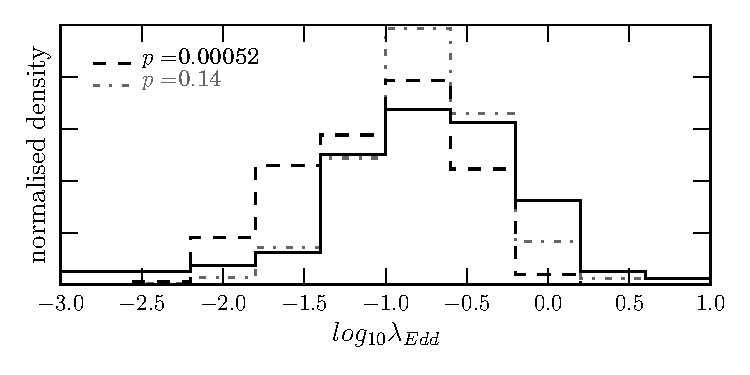
\includegraphics[width=0.8\textwidth]{agn/edd_ratio_z_matched_shen_2011_compare.pdf}
\caption[Eddington ratio distribution of the bulgeless AGN sample]{Normalised distributions of logarithmic Eddington ratio for the sample of 101 disc dominated galaxies (solid line), compared with that for the redshift matched sample from Shen et al. (2011; dashed line) and the entire sample (dot-dashed line) We also provide the p-values of a 2 sample KS test between the disc dominated sample and each of the quasar samples. We reject the null hypothesis that the two samples are drawn from the same population for the redshift matched quasar sample but accept the null hypothesis for the entire quasar sample of \citet{shen11}.  
}
\label{fig:eddratioshen}
\end{figure}


\begin{figure}
\centering
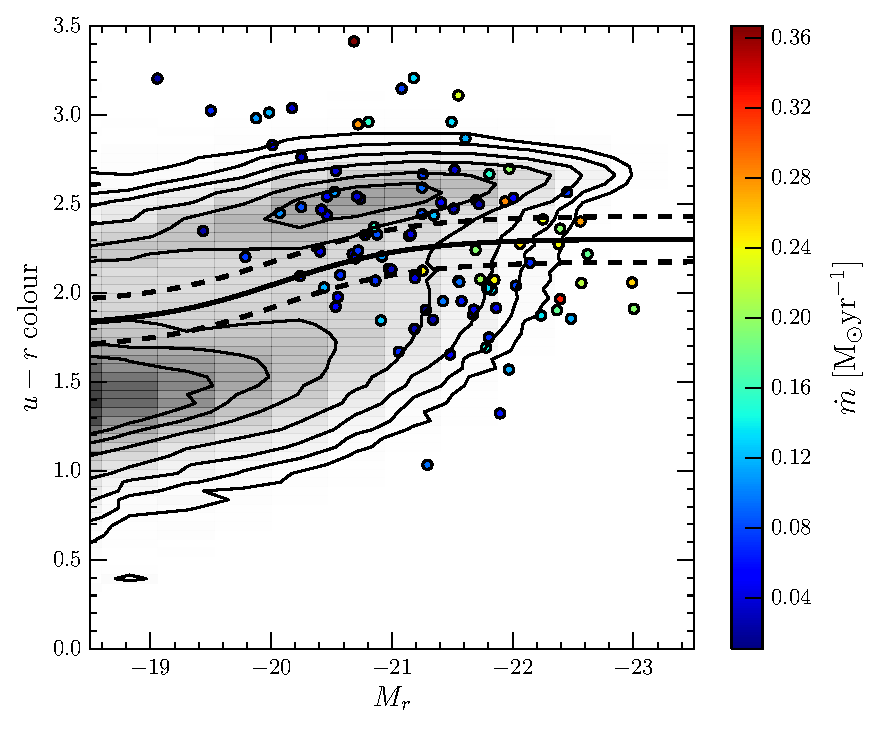
\includegraphics[width=\textwidth]{agn/CMD_DISCDOM_coloured_accretion_rate.pdf}
\caption[Colour-magnitude diagram for the DISCDOM sample, coloured by black hole mass accretion rate]{Optical colour-magnitude diagram showing the positions of the \textsc{discdom} sample (circles) in comparison to the SDSS DR7 sample from \citet{Baldry04}. The galaxies of the \textsc{discdom} sample are coloured by their black hole mass accretion rate, $\dot{m}$ (see Equation \ref{eq:mdot}). The definition between the blue cloud and red sequence  from \citet{Baldry04} is shown by the solid line (as defined in Equation~\ref{eqgv}) with $\pm~1\sigma$ shown by the dashed lines. The \textsc{discdom} sample are found across the colour magnitude diagram, however those with higher mass accretion rates are found preferentially in the green valley and at brighter r-band magnitudes.}
\label{fig:cmdmdot}
\end{figure}


%%%%%%%%%%%%%%%%%%%%%%%%%%%%%%%%%%%%%%%%%%%%%%
%
%  
\subsection{Discussion}\label{sec:intdiscussion}
%
%
%%%%%%%%%%%%%%%%%%%%%%%%%%%%%%%%%%%%%%%%%%%%%%


The relatively large number of purely disc galaxies of the \textsc{discdom} sample hosting growing SMBHs provides a very powerful probe of the simultaneous evolution of galaxies and their black holes driven without typical bulge-forming mechanisms. Despite the rarity of the morphology of these \textsc{discdom} galaxies, they are found in common areas of black-hole-galaxy scaling relations, as seen in Figures~\ref{fig:totvsbh}, \ref{fig:bulgevsbh} \& \ref{fig:mbhvsbol}, frequented by typical AGN host galaxies of all morphologies (they also lie in the common regions of the local $M_{BH}-\lambda_{Edd}$ plane shown in Figure 1 of the review paper of \citealt{alexander12}). Significant black hole growth has occurred up to masses of $M_{BH}\sim10^8 - 10^9~\rm{M}_{\odot}$ in the \textsc{discdom} sample whilst the disc dominated nature of the galaxy has been preserved. Simulations have repeatedly shown that mergers with mass ratios larger than 1:10 (i.e. mergers where the mass of the satellite is greater than $10\%$ of the main galaxy's mass) will form a classical bulge \citep{walker96, hopkins11c, tonini16}; so how is this substantial mass growth possible in the absence of such a major merger dominated (and minor merger limited) formation history?

Using Equation~\ref{eq:mdot}, the black hole mass accretion rates are estimated to lie in the range $0.01 \leq \dot{m} \leq 0.37 ~\rm{M}_{\odot}~\rm{yr}^{-1}$. Simulations by \citet{crockett11}, and more recently by \citet{diteodoro14}, show that such accretion rates are completely achievable by cold accretion of minor satellites with mass ratios less than 1:10 (i.e. the mass of the satellite galaxy is less than $10\%$ of the main galaxy mass). However, there is also evidence that such accretion rates may also be possible via merger free, secular processes alone. One such secular process, is bar driven gas inflow into the central regions of galaxies. Simulations of barred galaxies have repeatedly shown that gas inflow rates due to a morphological bar range from $\sim0.1-\rm{few} ~\rm{M}_{\odot}~\rm{yr}^{-1}$ \citep{sakamoto96, maciejewski02, regan04, lin13} and may increase to up to $\sim 7 ~\rm{M}_{\odot}~\rm{yr}^{-1}$ \citep{friedli93} with increasing bar length, bar strength and axis ratio. 

These simulations however, struggle to show that the gas funnelled to the central regions of the galaxy is actually accreted into the central few parsecs, and instead often accumulates in a nuclear ring wherein it causes a starburst \citep{regan04}. Similarly, no observational correlation has yet been found between the presence of a bar and and that of an AGN either locally \citep{ho97, malkan98, erwin02, lee12,cisternas13} or out to $z\sim1$ \citep{cheung15}. I estimate a bar fraction, $f_{\rm{bar}}$ in the \textsc{discdom} sample (which is by no means complete), by visual inspection of the SDSS ugriz images (see Figure~\ref{fig:exampleimages}), of $f_{\rm{bar}} \sim 0.42$; a lower limit due to the edge on nature of some of the galaxies in the \textsc{discdom} sample. In agreement with the studies above, this is no higher than the local bar fraction observed in the general local galaxy population \citep{masters11a}.

Using these derived black hole mass accretion rates, the time required to grow the black holes in the \textsc{discdom} sample from a seed mass of $10^2 ~\rm{M}_{\odot}$ can also be derived. This calculation assumes that the black holes have grown at the currently observed bolometric luminosity, since the mass at which that luminosity was the Eddington luminosity and prior to this underwent Eddington limited growth. This means that the accretion rates calculated, $\dot{m}$, will be the maximum rates at which the black holes have grown over their lifetimes. This is a conservative assumption but gives an estimate of the total time these black holes would need to spend in actively growing phase if the calculated rates are typical of black holes residing in disc dominated host galaxies. The mean (median) time taken for the black holes of the \textsc{discdom} sample to grow from a seed black hole mass is $\sim 1.68 ~\rm{Gyr}$ ($\sim 0.37 ~\rm{Gyr}$). These times are considerably less than a Hubble time, with the SMBHs in the \textsc{discdom} sample needing to spend only $\sim 10\%$ of their lifetimes in a growing phase to give the black hole masses currently measured. This is in agreement with the fraction of time predicted by simulations and observed by others \citep{kauffmann03, hao05, hopkins06, fiore12, Simmons13}.

A time of $\sim 38 ~\rm{Gyr}$ was calculated for two of the most massive black holes in the \textsc{discdom} sample, which have very low current Eddington ratios (see Figure~\ref{fig:mbhvsbol}). Since this time frame is well beyond the current estimates for the age of the Universe \citep[$\sim13.8 ~\rm{Gyr}$;][]{planck16}, this value is clearly an overestimate of the time taken to grow these two black holes. Since AGN are believed to go through a duty cycle of varying accretion rates throughout their lifetimes \citep{martini01, yu02, schawinski15}, then we can assume that these two black holes were accreting at a higher rate at some point in their history. If these two black holes are assumed to have grown within the median (mean) time derived for the rest of the \textsc{discdom} sample, then the past accretion rate will have been on the order of, $\dot{m} \sim 7.95 ~(1.73) ~\rm{M}_{\odot}~\rm{yr}^{-1}$. As discussed earlier, similar gas inflow rates caused by the presence of a bar have been seen in simulations \citep{friedli93}; suggesting once again that despite having large masses, these black holes could in theory be grown by secular processes. Unfortunately, the two host galaxies are at too high a redshift to allow the detection of a morphological bar in the SDSS ugriz image. 

The black hole mass accretion rates are also shown in Figure~\ref{fig:cmdmdot}, wherein the locations of the \textsc{discdom} sample on the optical colour magnitude diagram are shaded by $\dot{m}$. Those galaxies hosting black holes with higher mass accretion rates are found preferentially in the green valley and at brighter r-band magnitudes. This once again supports the arguments of Section~\ref{sec:agnfeedback} that feedback from these AGN could cause galaxies to quench, and therefore transition through the green valley, due to a sustained period of high mass accretion.

Figures~\ref{fig:mbhvsbol} \& \ref{fig:eddratioshen} show how the Eddington ratios of the \textsc{discdom} sample are higher than those in the bulge dominated \textsc{qsocontrol} sample (which has mean combined spiral vote fraction from GZ1 of $\left<p_{CS} \right> = 0.17$), so that the null hypothesis that the two Eddington ratio distributions are drawn from the same parent sample can be rejected. However, the same null hypothesis cannot be rejected for the full non-redshift matched AGN sample of \citet{shen11} which spans a redshift range of $0.06 < z < 5.46$. The Eddington ratios of the \textsc{discdom} sample are therefore higher than bulge dominated systems in the same redshift range, and instead are consistent with black hole accretion rates occuring at earlier cosmic times. So, despite having merger free evolutionary histories, black hole growth in the \textsc{discdom} galaxies is occurring at a higher rate than in typical local AGN host galaxies.  

The black hole masses of the disc dominated host galaxies in the \textsc{discdom} sample are not expected to correlate in the same way to their stellar masses as those in bulge dominated galaxies, if different dynamical histories lead to different mechanisms for black hole growth. However, Figure~\ref{fig:totvsbh} shows how the black hole and total stellar masses of the \textsc{discdom} sample occupy the same region of parameter space as the bulge dominated elliptical galaxies used to derive the \citet{haringrix04} relationship. Similarly Figure~\ref{fig:bulgevsbh} shows how the black hole masses of the \textsc{discdom} sample (which contain either no bulge, or a possible small pseudo bulge) lie well above the \citet{haringrix04} relationship, particularly when the upper limits on \textsc{discdom} bulge masses are taken into account. In other words, given what we know about black hole growth mechanisms, the black holes in these disc dominated systems are $\sim1-2~\rm{dex}$ more massive than they should be, given the mass (or lack thereof) of their bulge component. 

This is in agreement with the results of \citet{Simmons13} who found a similar excess in the black hole masses of $\sim 1.5~\rm{dex}$ and $\sim 2~\rm{dex}$ for the two measured black hole masses in their sample of 13 pure disc galaxies. Both this result and the results shown in Figures~\ref{fig:totvsbh} \& \ref{fig:bulgevsbh} at first seem to be in contradiction with previous works which find that galaxies with pseudo-bulges have lower black hole masses than predicted by typical scaling relations \citep[see work by][]{greene08, hu09, jiang11a, mathur12, ho14}. However, all these studies are biased by their sample selection methods, first selecting based on black hole mass to produce a sample of low mass black holes ($M_{BH} < 10^6 ~\rm{M}_{\odot}$) within which they hoped to find bulgeless or pseudo-bulge morphologies. Now, with the larger \textsc{discdom} sample shown in Figure~\ref{fig:bulgevsbh}, we can see that the fitted relationship between their black hole masses and bulge mass upper limits (solid black line), intersects with the relationship derived for the bulge dominated \citet{haringrix04} sample at $M_{BH} \sim 10^{6.4} ~\rm{M}_{\odot}$. At this point, the relationship predicts that for disc dominated galaxies the black hole masses will indeed be less than those predicted for bulge dominated systems, as concluded by the studies referenced above. 

Splitting the AGN host population by morphology in this way however, leads to biased conclusions. As discussed in Chapter~\ref{morph}, the strength of the \textsc{popstarpy} method lies partly due to the fact that no thresholds are applied to the GZ morphological vote fractions, allowing the dominance of intermediate quenching rates across the colour magnitude diagram to be revealed (see Section~\ref{sec:morphresults}). Similarly, if one does not ``\emph{discriminate}'' against morphology in the black hole mass-bulge mass plane and fit a linear regression model to galaxies in both the \textsc{discdom} (with proper consideration of upper limits) and \citet{haringrix04} samples, the result is consistent with a vertical line in the bulge-black hole mass plane. This suggests that there is perhaps no intrinsic correlation between black hole mass and stellar bulge mass across the full morphological spectrum of galaxies. 

This argument is supported by the agreement in Figure~\ref{fig:totvsbh} between the relationships derived in the total stellar mass-black hole mass plane for the \textsc{discdom} and bulge dominated \citet{haringrix04} samples. This agreement arises despite the two extremes in galaxy formation histories. This indicates that the mechanisms driving the dynamical and morphological structure of the galaxy may not be fundamental to the growth of the black hole. The black hole-galaxy relations observed across the $M_{BH}$-$\sigma$, $M_{BH}$-$M_{\rm{bulge}}$ and $M_{BH}$-$M_{*}$ planes, although demonstrating a correlation, have never implied a \emph{causation}. All of these parameters however, share mutual correlations to the overall gravitational potential of the dark matter halo of the galaxy \citep{booth10, volonteri11}, suggesting the true cause of the black-hole galaxy scaling relations is an outcome of hierarchical galaxy evolution \citep{jahnke11}, regardless of the merger history of the galaxy. 
 

\section{Conclusions}\label{sec:agnconclusion}

In Section \ref{sec:agnfeedback} I used morphological classifications from the Galaxy Zoo 2 project to determine the morphology-dependent SFHs of a population of $1,244$ Type 2 Seyfert AGN host galaxies, in comparison to an inactive galaxy population, via a Bayesian analysis of an exponentially declining SFH model. Using \textsc{popstarpy} I determined the population densities for the time and exponential rate that quenching occurs and find clear differences in the distributions, between \textsc{inactive} and \textsc{agn-host} galaxy populations and for host galaxies with AGN of different Eddington ratios. The main findings were:

\begin{enumerate}[(i)]
\item Quenching at early times is observed within the \textsc{inactive} population (see right panels of Figure~\ref{time}), where the population density is roughly constant until recent times where the distribution drops off at earlier times with increasing mass. This is evidence of downsizing within the \textsc{inactive} galaxy population, which is also seen in the \textsc{agn-host} smooth weighted population. This implies that AGN feedback is not responsible for the cessation of star formation within a proportion of these galaxies, as this quenching has occurred prior to the triggering of the current AGN.

\item Slow, early quenching is also observed in the disc weighted \textsc{agn-host} population (dashed lines bottom left panels of Figures~\ref{time} \& \ref{rate}) and so this SFH challenges the typical merger driven co-evolution of luminous black holes and their host galaxies.

\item Rapid quenching, possibly caused by the AGN itself through negative feedback, is the most dominant history within the low mass (left top panel Figure~\ref{rate}) and high Eddington ratio (bottom left panel of Figure~\ref{eddratiosplit}) \textsc{agn-host} population. This quenching history is particularly apparent for the smooth-weighted \textsc{agn-host} population, supporting the hypothesis that a merger, having caused a morphological transformation to a smooth galaxy, can also trigger an AGN, causing feedback and cessation of star formation on rapid timescales (initially proposed in Chapter~\ref{morph}). Further work is required to determine if the AGN is indeed the cause of the quenching seen. 

\item The prevalence of star forming AGN host galaxies, combined with the dominance of rapid, recent quenching seen across the \textsc{agn-host} population allows us to consider that either: (i)  the AGN are the cause of the rapid quenching observed but only in gas-poor host galaxies where they can have a large impact, (ii) the AGN are a consequence of another quenching mechanism but can also be triggered by other means which do not cause quenching, or (iii) the SFR of a galaxy can recover post-quench and return to the star forming sequence after a few Gyr.

\end{enumerate}

In Section \ref{intbulgeless} I studied how black holes can grow in galaxies with merger free evolutionary histories, by investigating where AGN in disc dominated galaxies lie on typical black-hole galaxy scaling relations. Despite the fact that these disc dominated galaxies have different dynamical histories to bulge-dominated and elliptical shaped systems, they are found to lie in the same regions of parameter space are $\sim1-2~\rm{dex}$ more massive than they should be, given the mass (or lack thereof) of their bulge component. The main findings were:
\begin{enumerate}[(i)]
\item Significant black hole growth has occurred up to masses of $M_{BH}\sim10^8 - 10^9~\rm{M}_{\odot}$ in the \textsc{discdom} sample whilst the disc dominated nature of the galaxy has been preserved.

\item Eddington ratios of the \textsc{discdom} sample are higher than those in the bulge dominated \textsc{qsocontrol} sample; despite having merger free evolutionary histories, black hole growth in the \textsc{discdom} galaxies is occurring at a higher rate than in typical local AGN host galaxies. 

\item Those galaxies hosting black holes with higher mass accretion rates are found preferentially in the green valley and at brighter r-band magnitudes. This once again supports the arguments of Section~\ref{sec:agnfeedback} that feedback from these AGN could cause galaxies to quench, and therefore transition through the green valley, due to a sustained period of high mass accretion.

\item Figures~\ref{fig:totvsbh} \& \ref{fig:bulgevsbh} show how the galaxies of the \textsc{discdom} sample occupy the same region of the $M_*$-$M_{\rm{BH}}$ and $M_{\rm{bulge}}$-$M_{\rm{BH}}$ parameter spaces, respectively, as the bulge dominated \citet{haringrix04} sample. Given what we know about black hole growth mechanisms, the black holes in these disc dominated systems are $\sim1-2~\rm{dex}$ more massive than they should be, given the mass (or lack thereof) of their bulge component. This suggests that there is perhaps no intrinsic correlation between black hole mass and galaxy bulge mass across the full morphological spectrum of galaxies and that the true cause of the black-hole galaxy scaling relations may be due to mutual correlations to the overall gravitational potential of the dark matter halo of the galaxy.


\end{enumerate}

It is therefore clear that AGN can have a large impact on the evolution of their host galaxies, including causing quenching directly through AGN feedback across the entire population; which I have demonstrated here for the first time. 

